%% This Beamer template is based on the one found here: https://github.com/sanhacheong/stanford-beamer-presentation, and edited to be used for Stanford ARM Lab

\documentclass[10pt]{beamer}
%\mode<presentation>{}

\usepackage{media9}
\usepackage{amssymb,amsmath,amsthm,enumerate}
\usepackage[utf8]{inputenc}
\usepackage{array}
\usepackage[parfill]{parskip}
\usepackage{graphicx}
\usepackage{caption}
\usepackage{subcaption}
\usepackage{bm}
\usepackage{amsfonts,amscd}
\usepackage[]{units}
\usepackage{listings}
\usepackage{multicol}
\usepackage{multirow}
\usepackage{tcolorbox}
\usepackage{physics}
%encoding
%--------------------------------------
\usepackage[T1]{fontenc}
\usepackage[utf8]{inputenc}
%--------------------------------------

%Portuguese-specific commands
%--------------------------------------
\usepackage[portuguese]{babel}
%--------------------------------------

%Hyphenation rules
%--------------------------------------
\usepackage{hyphenat}
\hyphenation{mate-mática recu-perar}
%--------------------------------------

% Enable colored hyperlinks
\hypersetup{colorlinks=true}

% The following three lines are for crossmarks & checkmarks
\usepackage{pifont}% http://ctan.org/pkg/pifont
\newcommand{\cmark}{\ding{51}}%
\newcommand{\xmark}{\ding{55}}%

% Numbered captions of tables, pictures, etc.
\setbeamertemplate{caption}[numbered]

%\usepackage[superscript,biblabel]{cite}
\usepackage{algorithm2e}
\renewcommand{\thealgocf}{}

% Bibliography settings
\usepackage[style=ieee]{biblatex}
\setbeamertemplate{bibliography item}{\insertbiblabel}
\addbibresource{references.bib}

% Glossary entries
\usepackage[acronym]{glossaries}
\newacronym{ML}{ML}{machine learning}
\newacronym{HRI}{HRI}{human-robot interactions}
\newacronym{RNN}{RNN}{Recurrent Neural Network}
\newacronym{LSTM}{LSTM}{Long Short-Term Memory}


\theoremstyle{remark}
\newtheorem*{remark}{Remark}
\theoremstyle{definition}

\newcommand{\empy}[1]{{\color{darkorange}\emph{#1}}}
\newcommand{\empr}[1]{{\color{cardinalred}\emph{#1}}}
\newcommand{\examplebox}[2]{
\begin{tcolorbox}[colframe=darkcardinal,colback=boxgray,title=#1]
#2
\end{tcolorbox}}

\usetheme{Stanford} 
\def \i  {\item}
\def \ai {\item[] \quad \arrowbullet}
\newcommand \si[1]{\item[] \quad \bulletcolor{#1}}
\def \wi {\item[] \quad $\ \phantom{\Rightarrow}\ $}
\def \bi {\begin{itemize}\item}
\def \ei {\end{itemize}}
\def \be {\begin{equation*}}
\def \ee {\end{equation*}}
\def \bie {$\displaystyle{}
\def \eie {{\ }$}}
\def \bsie {\small$\displaystyle{}
\def \esie {{\ }$}\normalsize\selectfont}
\def \bse {\small\begin{equation*}}
\def \ese {\end{equation*}\normalsize}
\def \bfe {\footnotesize\begin{equation*}}
\def \efe {\end{equation*}\normalsize}
\renewcommand \le[1] {\\ \medskip \lefteqn{\hspace{1cm}#1} \medskip}
\def \bex {\begin{example}}
\def \eex {\end{example}}
\def \bfig {\begin{figure}}
\def \efig {\end{figure}}
\def \btheo {\begin{theorem}}
\def \etheo {\end{theorem}}
\def \bc {\begin{columns}}
\def \ec {\end{columns}}
\def \btab {\begin{tabbing}}
\def \etab {\end{tabbing}\svneg\svneg}
\newcommand \col[1]{\column{#1\linewidth}}
\def\vneg  {\vspace{-5mm}}
\def\lvneg {\vspace{-10mm}}
\def\svneg {\vspace{-2mm}}
\def\tvneg {\vspace{-1mm}}
\def\vpos  {\vspace{5mm}}
\def\lvpos {\vspace{10mm}}
\def\svpos {\vspace{2mm}}
\def\tvpos {\vspace{1mm}}
\def\hneg  {\hspace{-5mm}}
\def\lhneg {\hspace{-10mm}}
\def\shneg {\hspace{-2mm}}
\def\thneg {\hspace{-1mm}}
\def\hpos  {\hspace{5mm}}
\def\lhpos {\hspace{10mm}}
\def\shpos {\hspace{2mm}}

\logo{
\includegraphics[height=0.4in]{./images/logoufjf10.png}}

% commands to relax beamer and subfig conflicts
% see here: https://tex.stackexchange.com/questions/426088/texlive-pretest-2018-beamer-and-subfig-collide
\makeatletter
\let\@@magyar@captionfix\relax
\makeatother

\newcommand{\code}[1]{\textcolor{red} {\textit{#1}}} %comentarios

\title[Docker \& Qt]{Docker \& Qt}
%\subtitle{Subtitle Of Presentation}

%\beamertemplatenavigationsymbolsempty

\begin{document}

\author[Modelagem Computacional]{
	\begin{tabular}{c} 
	\Large
	Igor Pires dos Santos\\
    \footnotesize \href{mailto:igor.pires@ice.ufjf.br}{igor.pires@ice.ufjf.br}\\
    \textbf{Professor:} Bernardo M. Rocha
\end{tabular}
\vspace{-4ex}}

\institute{
	\vskip 5pt
	\begin{figure}
		\centering
		\begin{subfigure}[t]{0.5\textwidth}
			\centering
			
\includegraphics[height=0.33in]{images/logoufjf1}
		\end{subfigure}%
		~ 
		\begin{subfigure}[t]{0.5\textwidth}
			\centering
			
\includegraphics[height=0.33in]{./images/PGMC.png}
		\end{subfigure}
	\end{figure}
	\vskip 5pt
	Programa de Pós-Graduação em Modelagem Computacional\\
	Universidade Federal de Juiz de Fora\\
	\vskip 3pt
}

% \date{June 15, 2020}
\date{\today}

\begin{noheadline}
\begin{frame}\maketitle\end{frame}
\end{noheadline}

\setbeamertemplate{itemize items}[default]
\setbeamertemplate{itemize subitem}[circle]

\begin{frame}
	\frametitle{Sumário} % Table of contents slide, comment this block out to remove it
	\tableofcontents % Throughout your presentation, if you choose to use \section{} and \subsection{} commands, these will automatically be printed on this slide as an overview of your presentation
\end{frame}

\section{Docker - Introdução}
\begin{frame}[allowframebreaks]
\frametitle{Docker - Introdução}
	\begin{itemize}
		\item \textbf{O que é o Docker?}
		\item O Docker foi criado como um projeto \textit{open source}, em 2013, pela então nomeada DotCloud. Pouco mais de um ano após o lançamento do projeto a empresa passou por uma reestruturação.
		\item Isso se deu pela grandiosidade que o Docker tomou, englobando a empresa original e criando-se a Docker \texttrademark.
	\end{itemize}
	
	\framebreak
	
	\begin{itemize}
		\item Desde então diversas empresas mudaram seus sistemas de \textit{software management} para a estrutura Docker. Isso se dá pela praticidade em migrar e manter o sistema utilizando o Docker
		\item Especialistas da área dizem que grandes revoluções assim no meio da computação não inevitáveis, que as grandes empresas precisam se adaptar para correr atrás desta tecnologia ou serão devoradas.
		
	\end{itemize}
	
	\framebreak
	
	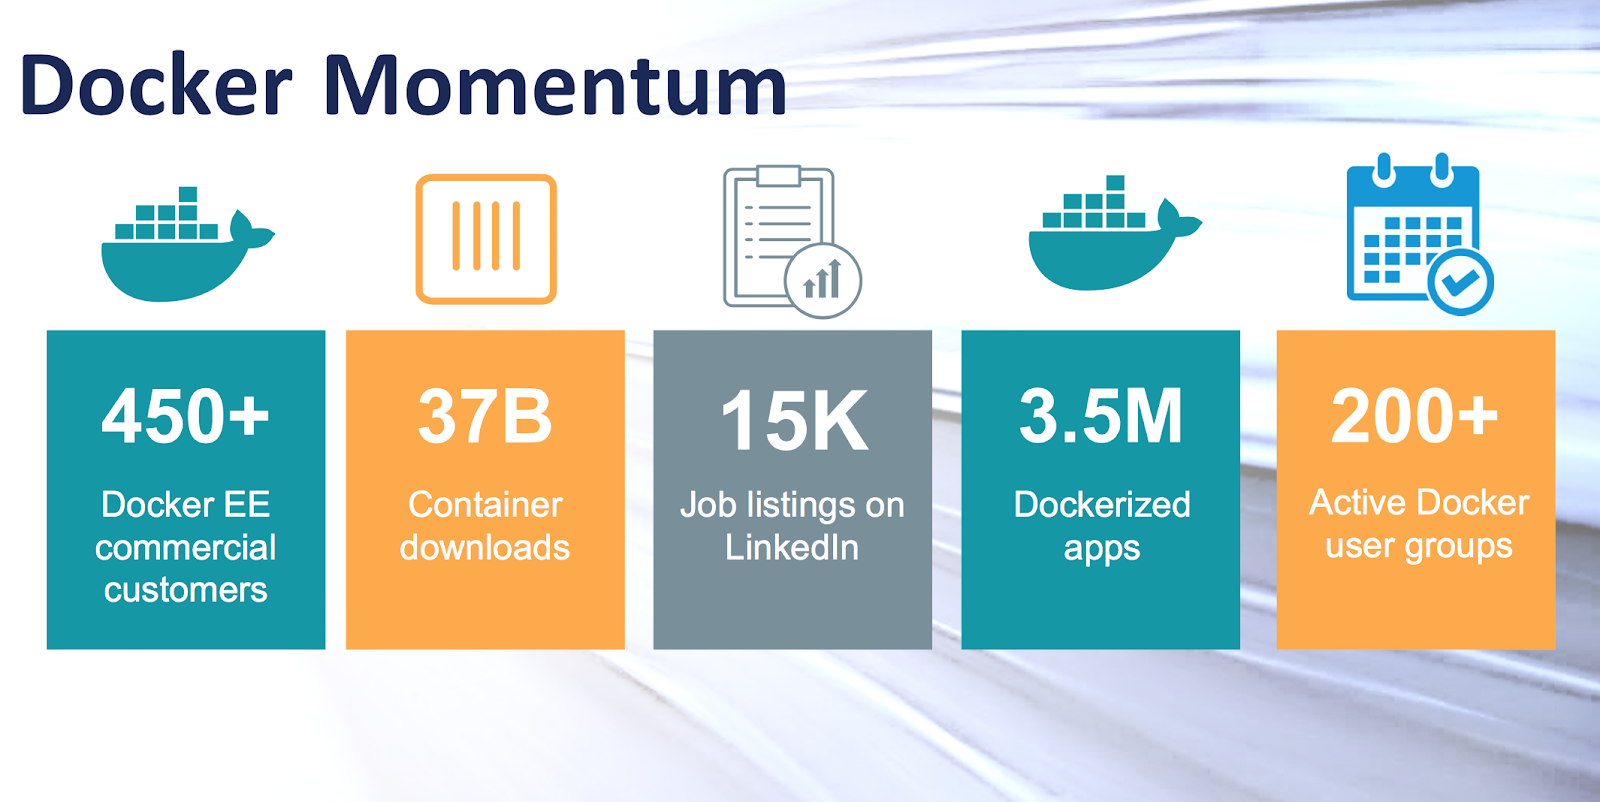
\includegraphics[width=1\textwidth]{images/01.jpg} 
	
	\framebreak
	
	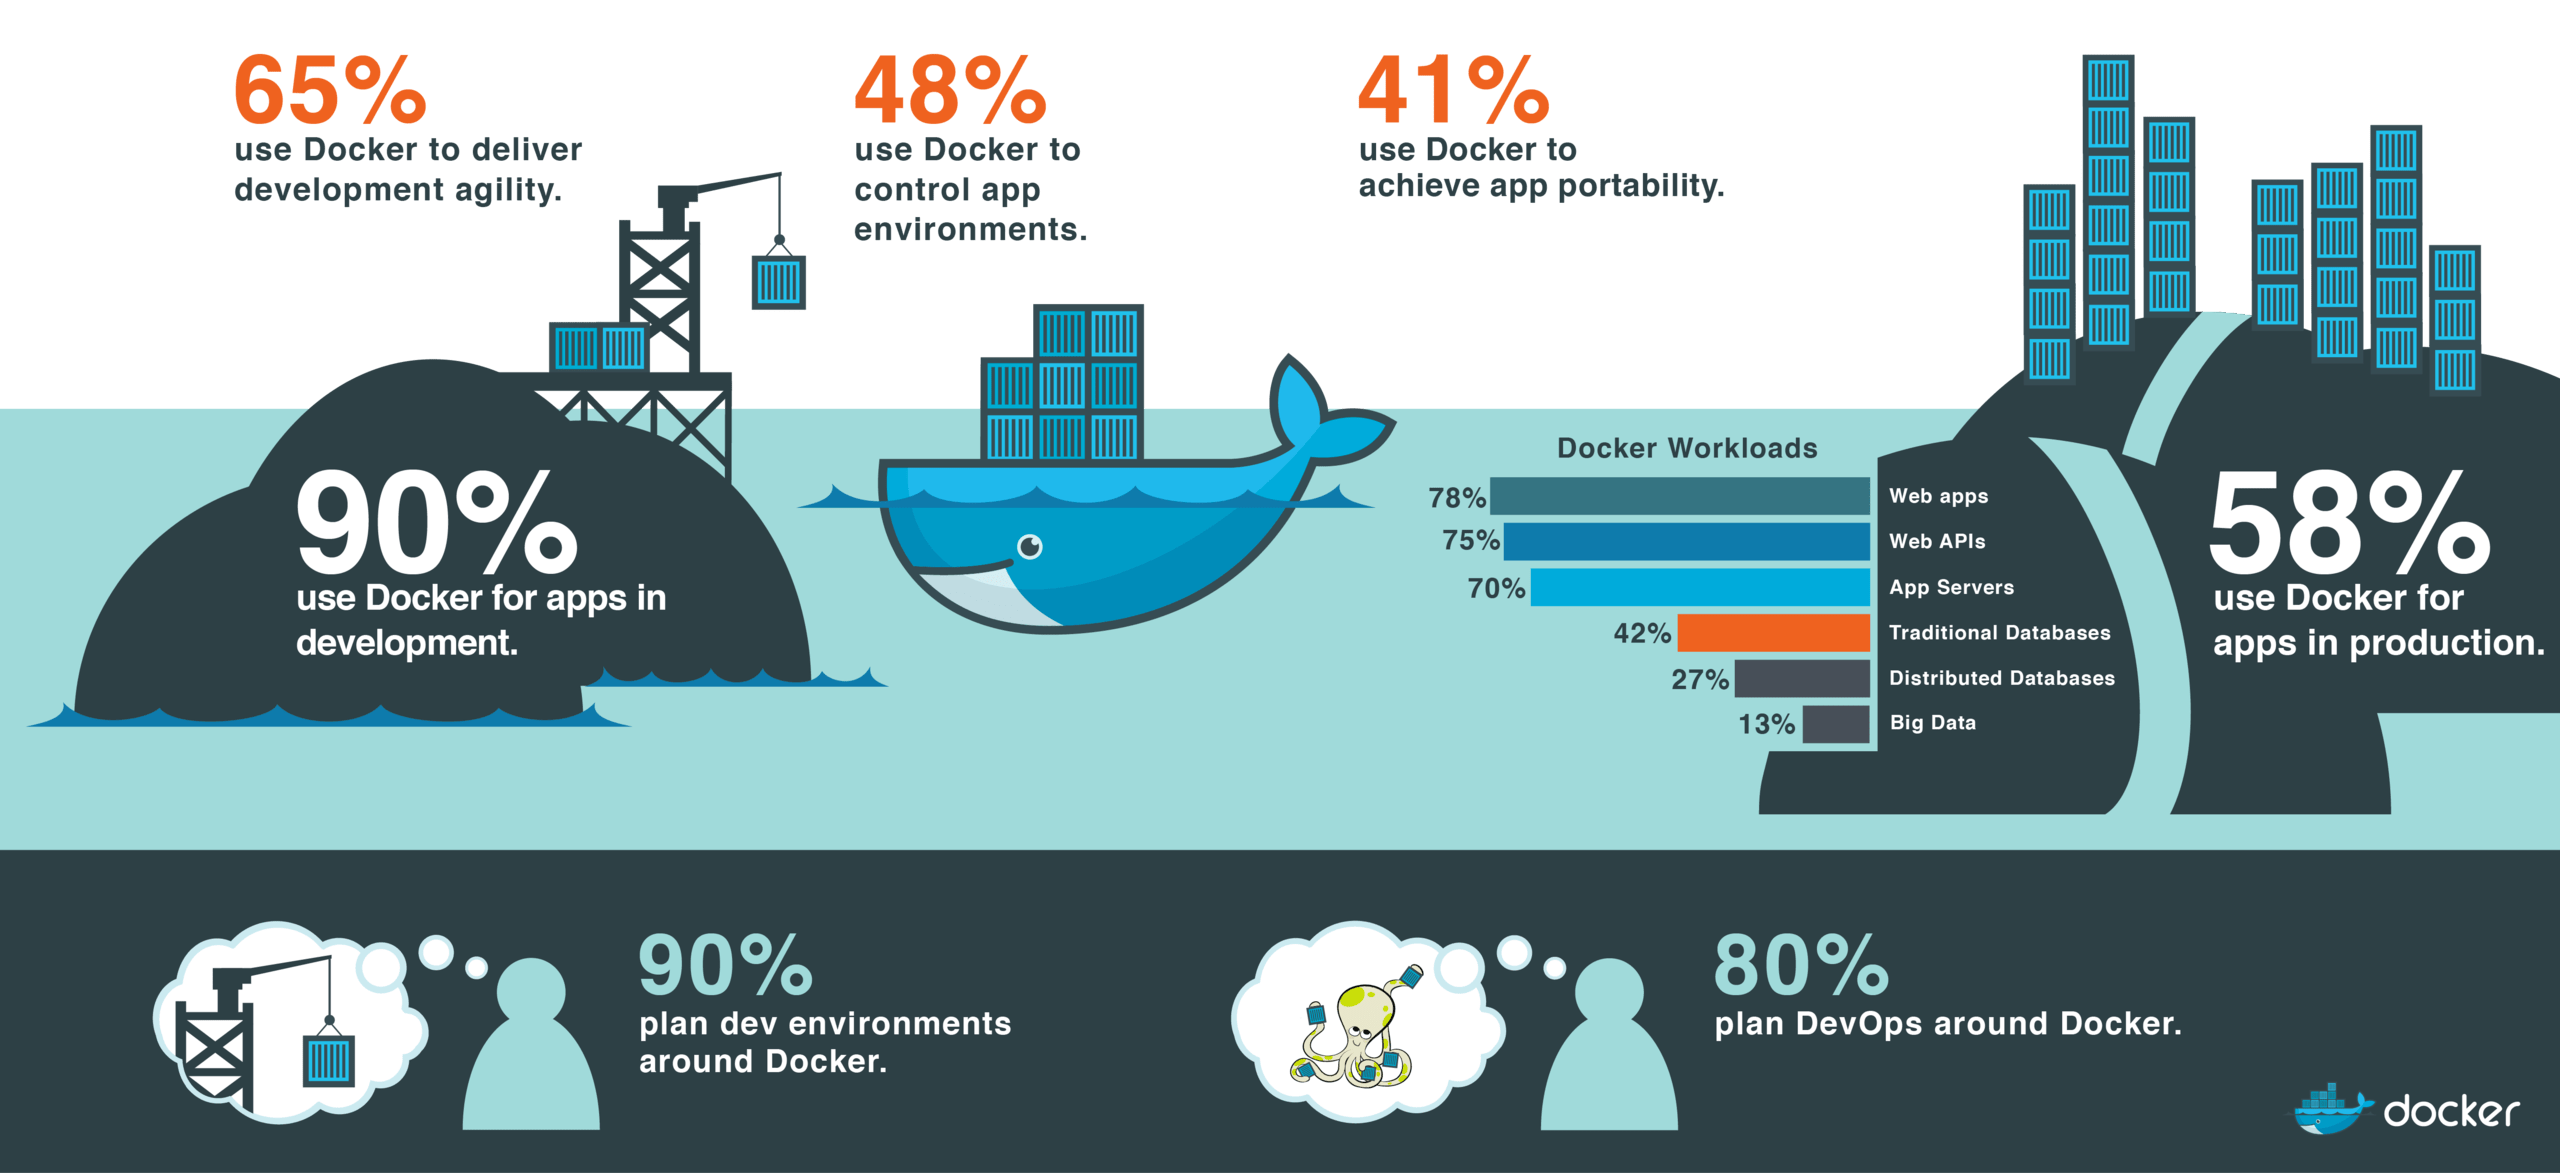
\includegraphics[width=1\textwidth]{images/Docker_Supply-chain-V1.5-01.png} 
	
	\framebreak
	
	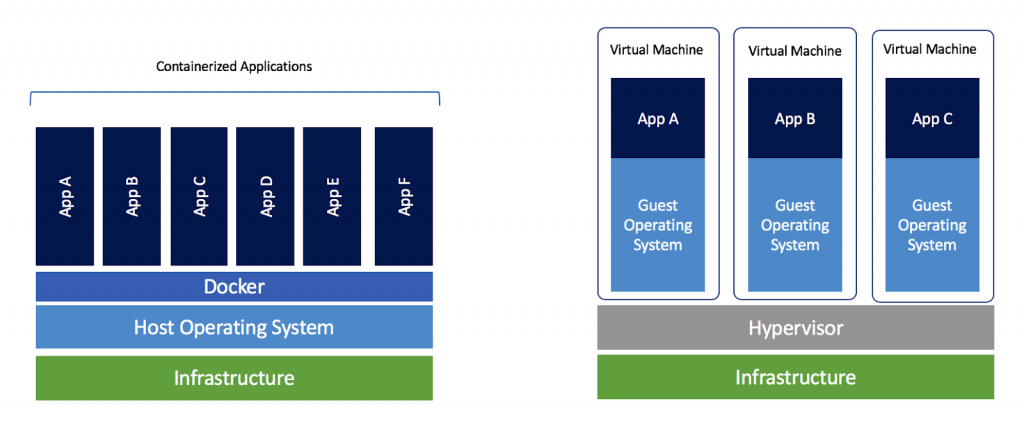
\includegraphics[width=1\textwidth]{images/02.jpg}
	
	\framebreak
	
	\begin{itemize}
		 \item Há algum tempo o Docker não é mais referenciado como uma alternativa à máquinas virtuas, ou contêineres em tempo de execução
		 \item O Docker assim como a maioria das tecnologias atuais está em constante evolução. Portanto, os materiais de referência ao Docker também estão em constante atualização. Existem diferentes versões da ferramenta Docker, aqui fala-se exclusivamente do Docker CE (Community Edition).
	 \end{itemize} 
	
\end{frame}


\section{Docker - Instalação}
\begin{frame}[allowframebreaks]
\frametitle{Docker - Instalação}

	\begin{itemize}
	\item Existem três tipos de instalação do Docker:
	
	\item \textbf{Direta}: A instalação direta significa que o Docker estará rodando diretamente no Sistema Operacional (SO) do ambiente utilizado. Instalando-se o Docker no Linux e suas distribuições os conteinêres estão rodando "\textit{nativamente}" e podem ser acessados diretamente pela linha de comando. Versões do Mac OSX acima de Yosemite 10.10.3 e o Windows 10 \textbf{Pro} possui uma tecnologia (\textit{Hyper-V}) que permite a utilização destes contêineres "\textit{nativos}". 
	
	\item \textbf{Mac/Windows}: Em outras versões do Windows e Mac o Docker utiliza de uma máquina virtual dentro dos SOs com Linux para poder rodar os contêineres.
	
	\item \textbf{Cloud}: Existem versões do Docker que são feitas expecificamentes para sistemas "nas nuvens", como Azure, AWS e Google. Com isto as empresas conseguem utilizar o Docker em Larga Escala.
	\end{itemize}
	
	\framebreak
	
	\begin{itemize}
		\item \textbf{Docker CE vs Docker EE}: Basicamente ao se adquirir a versão Enterprise do Docker o usuário é incluído no ciclo de vida do Docker e tem suporte para sua aplicação em específico além de produtos extras. Atualmente em 5 US\$ por mês.
		
		\item \textbf{Stable vs Edge}: Ao instalar o docker você pode selecionar dois tipos de versionamento. As funcionalidades inseridas na versão \textit{Stable} possuem suporte por maior tempo.
		
	\end{itemize}
	
	\framebreak
	
	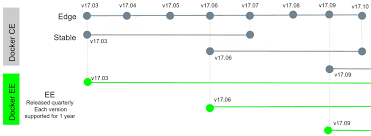
\includegraphics[width=1\textwidth]{images/02.png}
	
	\framebreak
	
	\begin{itemize}
		\item \textbf{Docker para Windows 10 Pro}
		
		\item Nesta versão do Windows existe a ferramenta "\textit{Docker Desktop}" que traz a melhor experiência do Docker no Windows, pois com a tecnologia Hyper-V que é uma virtualização nativa do Windows, sendo mais rápido que uma Máquina Virtual (MV) de fato.
		
		\item Nesta versão é possível acessar os comandos do Docker através do Powershell.
	\end{itemize}
	
	\framebreak
	
	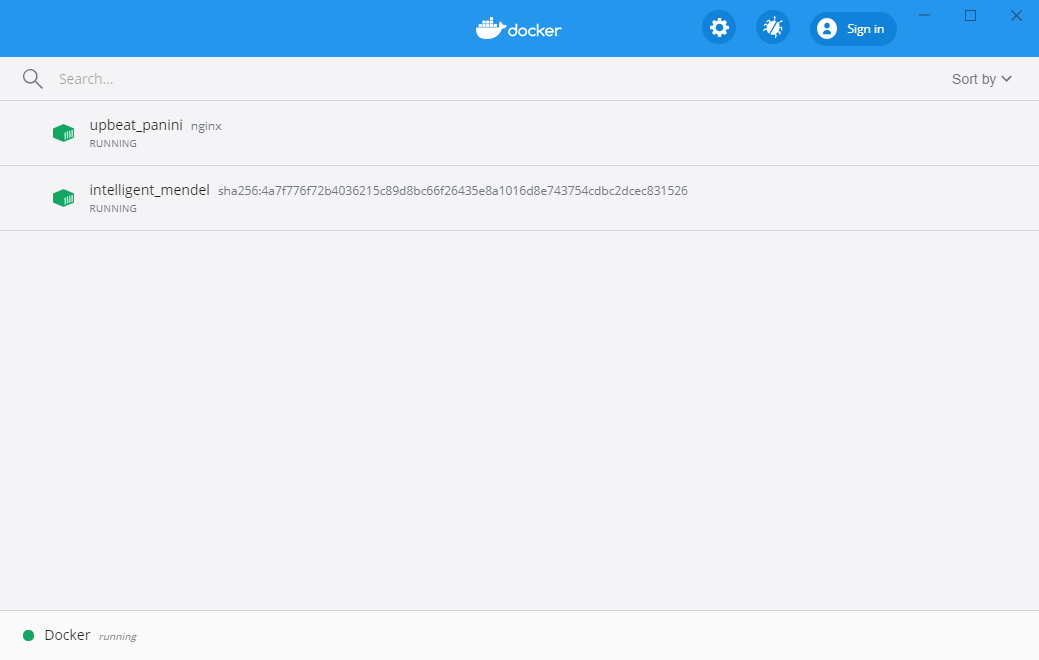
\includegraphics[width=1\textwidth]{images/10.png}
	
	\framebreak
	
	\begin{itemize}
		\item \textbf{Docker para Windows 7, 8, 10 Home}
		
		\item Infelizmente para estas versões do Windows não há tecnologia que permita os contêineres rodem "nativamente". Para estas versões é necessário instalar o Docker Toolbox, juntamente com algum gerenciador de MVs como o Oracle VirtualBox.
		
		\item Nesta versão é possivel acessar os comandos do Docker através de SSH com a máquina virtual criada.
	\end{itemize}
	
	\framebreak
	
	\begin{itemize}
		\item \textbf{Docker para Mac}
		
		\item Assim como no caso do Windows, existe a ferramenta "\textit{Docker Desktop}" com a versão nativa do Docker para OSX com versão superior à Yosemite 10.10.3 e \textit{Docker Toolbox} para as demais.
	\end{itemize}
	
	\framebreak
	
	\begin{itemize}
		\item \textbf{Docker para Linux}
		
		\item \textbf{Não} utilizar versões pré compiladas.
		
		\item  \textbf{Ubuntu e Distros grátis}: O comando abaixo utiliza de um script automatizado do Docker que instala todoas as dependências juntamente:
		
		\item \code{curl -sSL https://get.docker.com/ | sh}
		
		\item Todas as Distro Unix pagas requerem a versão EE do Docker.
		
		\item Todos os sistemas Unix com docker requerem a instalação separada dos pacotes "docker-compose" e  "docker-machine".
	\end{itemize}
	
	\framebreak
	
	\begin{itemize}
		\item \textbf{Docker Compose}:
		\item \code{sudo curl -L "https://github.com/docker/compose/releases/download/1.26.2/docker-compose-\$(uname -s)-\$(uname -m)" -o /usr/local/bin/docker-compose}
		\item \code{sudo chmod +x /usr/local/bin/docker-compose}
	\end{itemize}
	
	\framebreak
	
	\begin{itemize}
		\item \textbf{Docker Machine}:
		\item \code{base=https://github.com/docker/machine/releases/download/v0.16.0 \&\&  curl -L \$base/docker-machine-\$(uname -s)-\$(uname -m) >/tmp/docker-machine \&\&  sudo mv /tmp/docker-machine /usr/local/bin/docker-machine \&\&
  chmod +x /usr/local/bin/docker-machine}
	\end{itemize}
	
	\framebreak
	
	\begin{itemize}
		\item Com o Docker instalado, o seguinte comando pode ser executado:
		
		\item \code{docker version}
	\end{itemize}
	
	\framebreak
	
	\begin{center}
		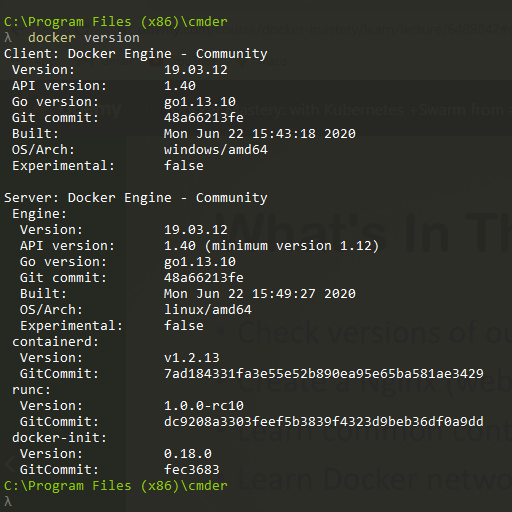
\includegraphics[width=0.6\textwidth]{images/03.png}
	\end{center}	
	
	
\end{frame}



\section{Docker - Contêineres}
\begin{frame}[allowframebreaks]
\frametitle{Docker - Contêineres}
		
	\begin{center}
		
\includegraphics[width=0.6\textwidth]{images/04.png}
	\end{center}
	
	\framebreak
	
	\begin{center}
		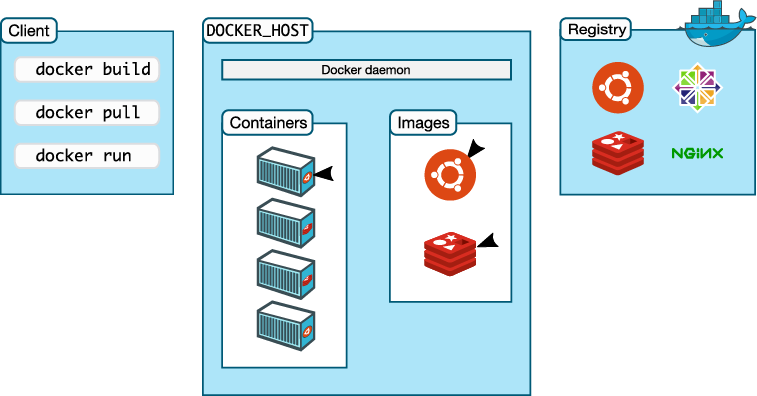
\includegraphics[width=0.6\textwidth]{images/01.png}
	\end{center}	
	
	\framebreak
	
\begin{itemize}
	\item 	Com a estrutura do Docker insalada no ambiente é possível então iniciar diretamente contêineres, como por exemplo um servidor Nginx:
	
	\item \code{docker container run nginx}

	\item Automaticamente ao se instalar o Docker se ganha acesso ao \textit{hub.docker.com} que é um repositório de imagens além das outras funcionalidades. Portanto, ao executar o comand,o a imagem "nginx" é "puxada" do repositório e executada no Docker
\end{itemize}
	
	\framebreak
	
	\begin{itemize}
		\item Quando o nome do contêiner é somente o seu nome como \code{nginx} significa que ele é gerido por uma empresa e tem o selo do Docker.
		
		\item Quando o nome do contêiner é \code{user/container} significa que algum usuário é o dono daquela imagem e ela não possui selo do Docker.
	\end{itemize}
	
	\framebreak
	
	\begin{center}
		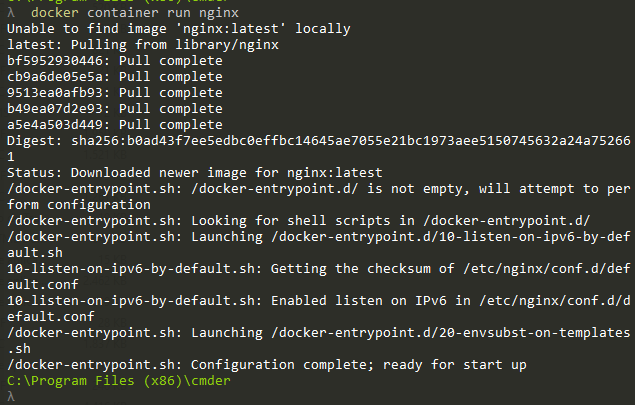
\includegraphics[width=0.6\textwidth]{images/07.png}
	\end{center}	
	
	\framebreak
	
	\begin{itemize}
		\item \textbf{Estrutura dos comandos}
		
		\item Todos os comandos do Docker seguem esta estrutura (\textit{fora os comandos mais antigos}):
		
		\item \code{docker <escopo> <comando>}
		
	\end{itemize}
	
	
	\framebreak
		
	\begin{center}
		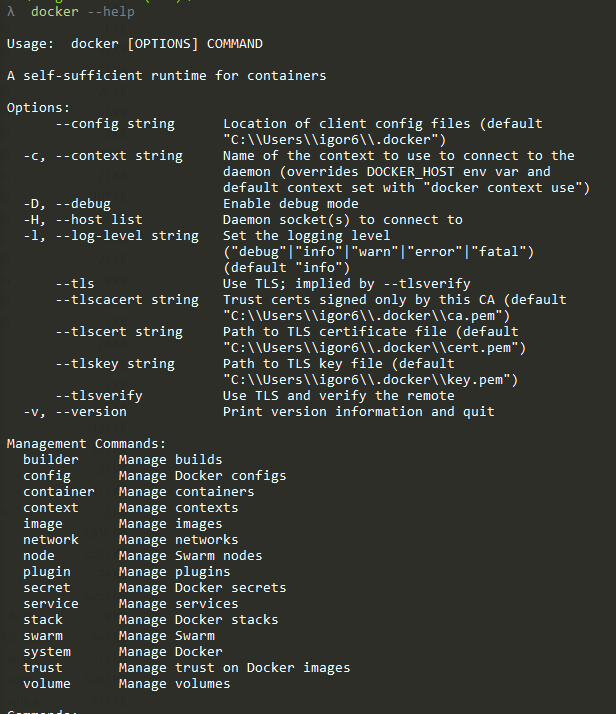
\includegraphics[width=0.6\textwidth]{images/05.png}
	\end{center}	
	
	\framebreak
		
	\begin{center}
		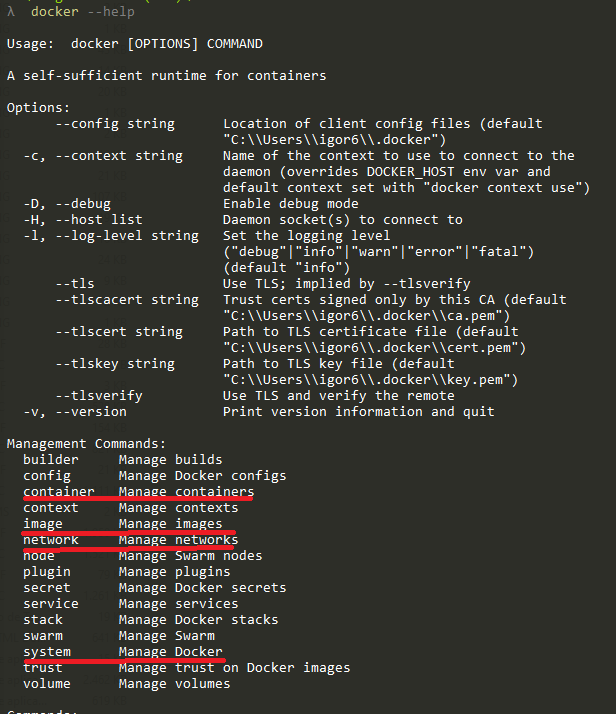
\includegraphics[width=0.6\textwidth]{images/06.png}
	\end{center}
	
	\framebreak	
	
	\begin{itemize}
		\item Após a execução do comando \code{docker container run ngnix} um contêiner é inicializado com a imagem incial de um servidor HTTP Nginx. Ao executar este comando o \textit{shell} dica preso à execução, mostrando o log de execução do contêiner até que \textit{Ctrl+C} seja pressionado ou o contêiner pare esnpotâneamente.
		
		\item Portanto para gerir bem o ambiente Docker e os recursos computacionais é necessário o acesso à imagens e contêineres armazenados, devido ao seu tamanho e custo computacional. O comando abaixo lista todos os contêineres:
		
		\item \code{docker container ls -a}
	\end{itemize}
	
	\framebreak
		
	\begin{center}
		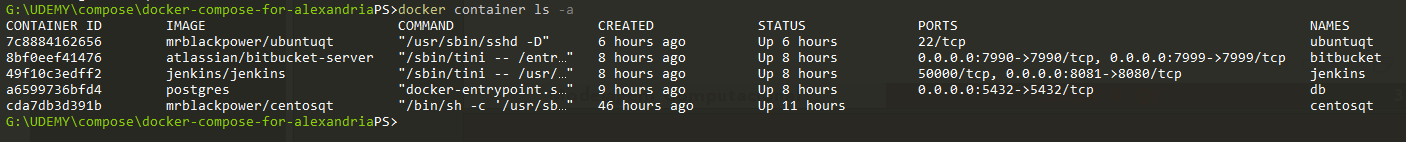
\includegraphics[width=1\textwidth]{images/11.png}
	\end{center}
	
	\framebreak
	
	\begin{itemize}
		\item Com o comando anterios é possível ver todos os contêineres, inclusive os parados. Para parar a execução de um contêiner utilizamos:
		
		\item \code{docker container stop <conteiner-id-list>}
		
		\item Analogamente, \code{docker container start <conteiner-id-list>} para reiniciar-los.
		
		\item E para removê-los:
		
		\item \code{docker container remove <conteiner-id-list>}
	\end{itemize}	
		
	\framebreak
	
	\begin{itemize}
		\item Além disso, portas do contêiner podem ser expostas localmente para que possamos acessar os dados através dos protocolos disponíveis.
		
		\item Pode-se iniciar o contêiner com a \textit{flag} -p:
		
		\item \code{docker container run -d -p 80:80 nginx}
	\end{itemize}
		
	\framebreak
		
	\begin{itemize}
		\item Desta forma, ao acessar o endereço \textcolor{blue}{http://localhost:80} a seguinte imagem deve aparecer.
	\end{itemize}		
		
	\begin{center}
		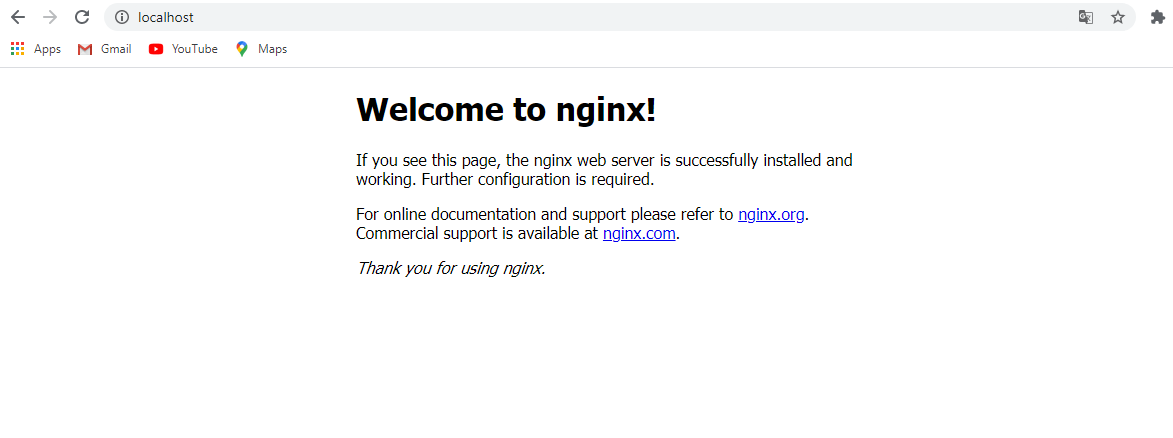
\includegraphics[width=1\textwidth]{images/13.png}
	\end{center}
	
\end{frame}

\section{Docker - Imagens}
\begin{frame}[allowframebreaks]
\frametitle{Docker - Imagens}
	
	\begin{itemize}
		\item Nesta seção analisaremos como o sitema de imagens do Docker e o ropositório de imagens Docker Hub funcionam.
		
		\item Como dito anteriormente as imagens são os dados de todo o contêiner, contendo o SO bem como os comandos realizados posteriormente.
		
		\item Portanto é possível fazer o download de uma imagem alterar os seus arquivos e subir novamente sua imagem.
		
		\item Para visualizar as imagens já armazenadas no cache do Docker, se utiliza o comando:
		
		\item \code{docker image ls -a}
	\end{itemize}
		
	\framebreak	
		
	\begin{center}
		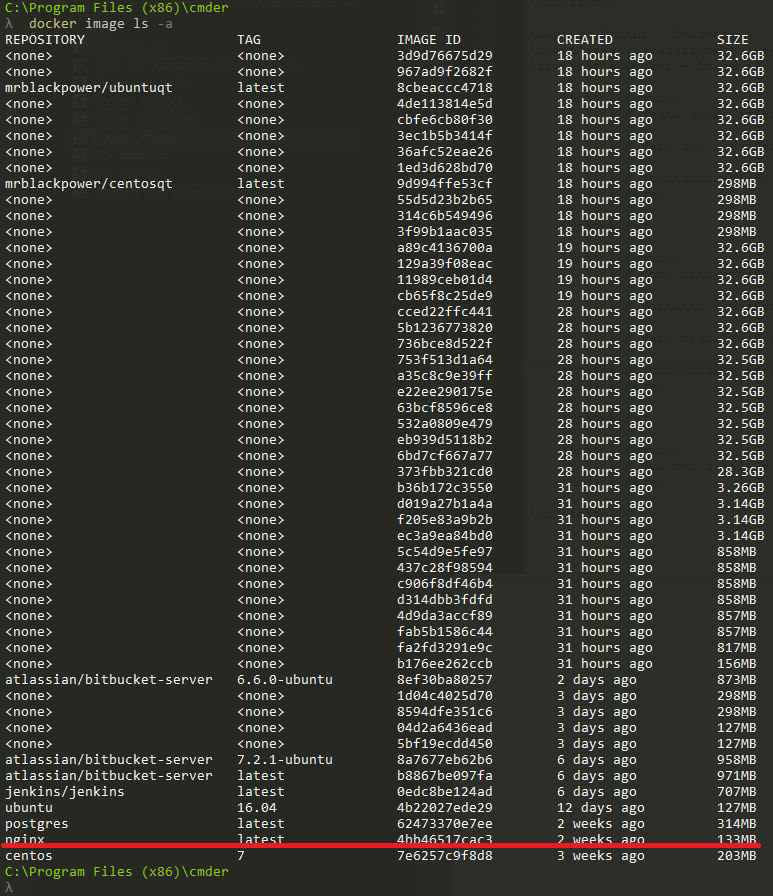
\includegraphics[width=0.6\textwidth]{images/14.png}
	\end{center}
			
	\framebreak	
	
	\begin{itemize}
		\item É possível ainda atualizar estas imagens atualizadas com o mais novo conteúdo do contêiner através do comando \code{docker container commit <container> <image:tag>}
	\end{itemize}
	
	\begin{center}
		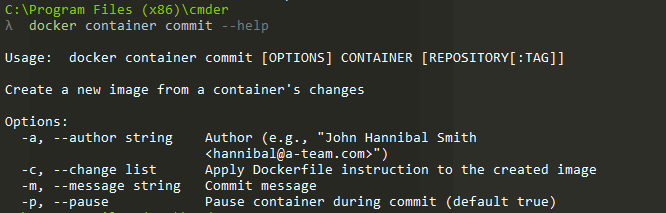
\includegraphics[width=0.6\textwidth]{images/17.png}
	\end{center}
	
	\framebreak

	\begin{itemize}
		\item O Docker Hub é um repositório de imagens que funciona em conjunto com o Docker. Assim como um repositório \textit{git} ele é responsável pelo gerenciamento de arquivos e o versoniamento, entretanto lida apenas com imagens Docker. Desta forma o repositório permite que rapidamente as imagens sejam salvas nas nuvens e utilizadas remotamente.
		
		\item Para que o repositório de imagens funcione corretamente é necessário criar uma conta no portal \textcolor{blue}{\textit{hub.docker.com}}
		
		\item \textcolor{blue}{\textit{https://hub.docker.com/signup}}
	\end{itemize}
		
	\framebreak
		
	\begin{center}
		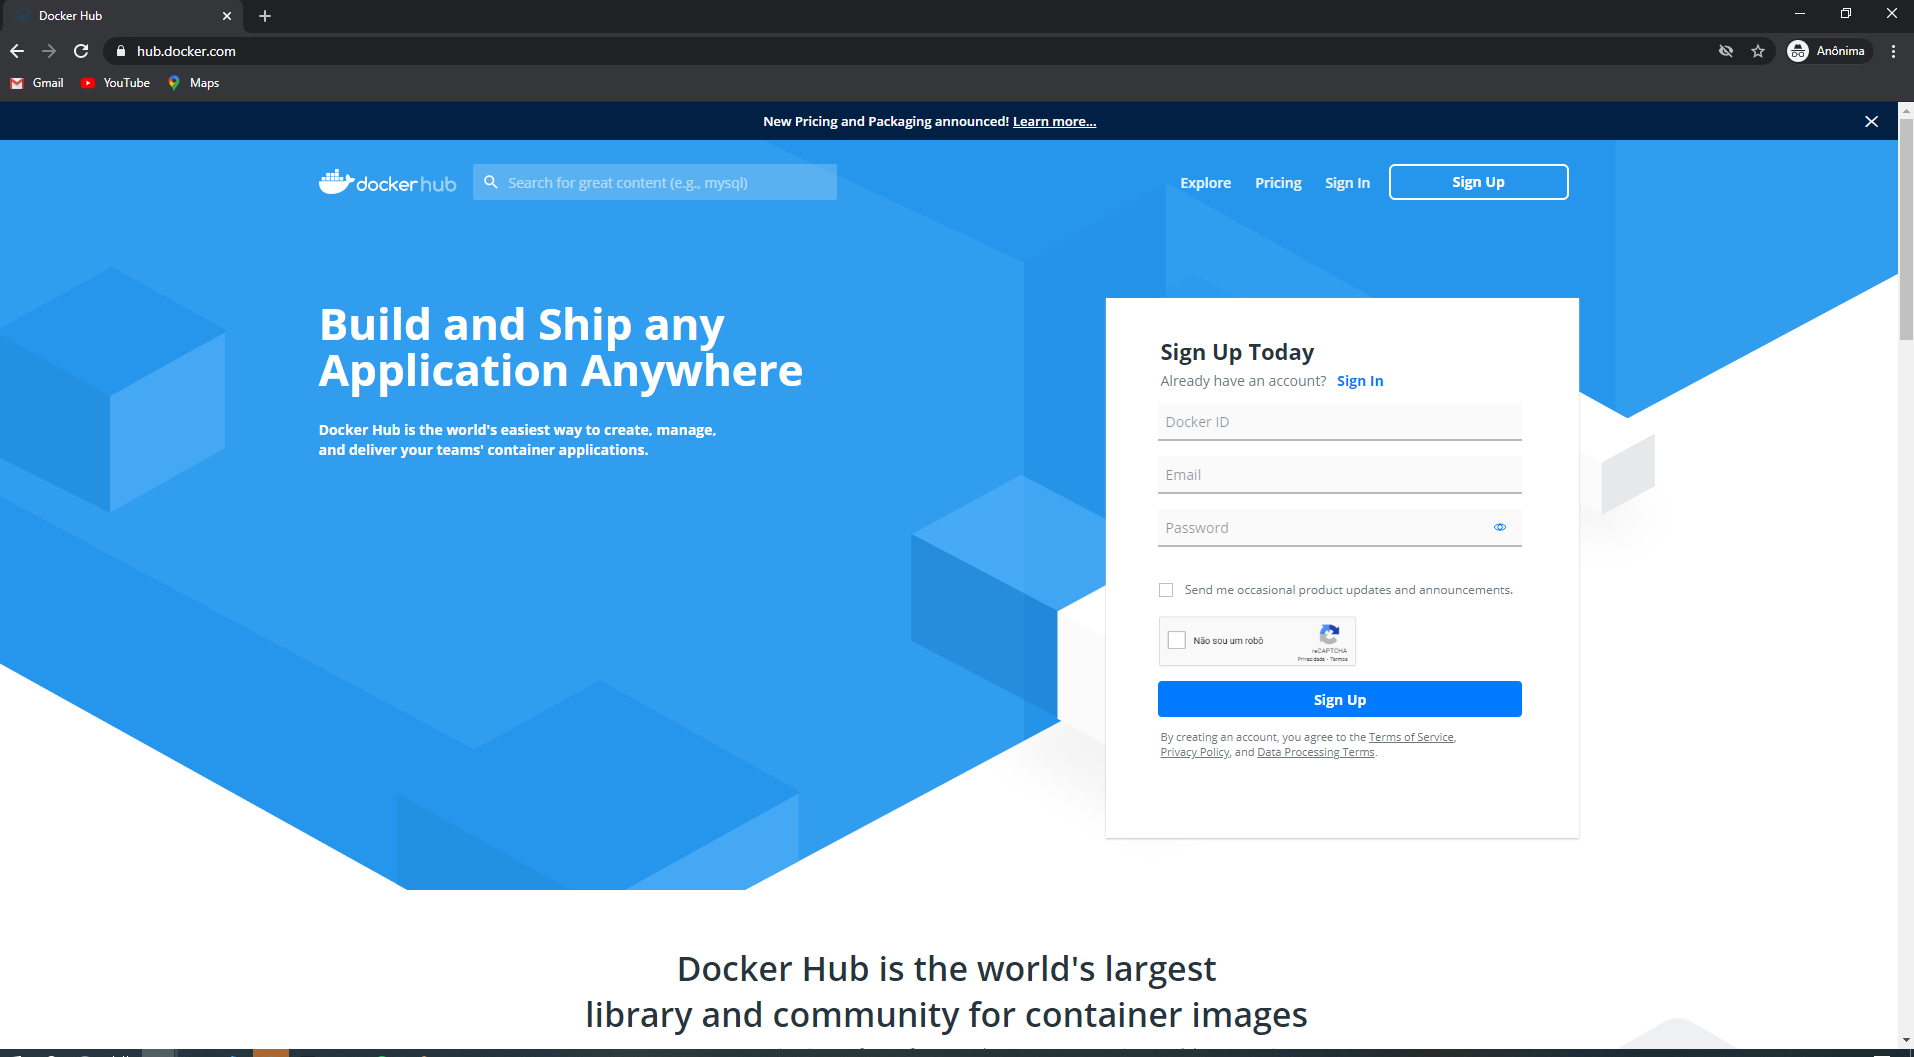
\includegraphics[width=1\textwidth]{images/15.png}
	\end{center}
	
	\framebreak
	
	\begin{itemize}
		\item Uma vez criada a conta é necessário que se faça o login antes de ter acesso ao repositório pessoal e ser possível "\textit{subir}" imagens.
		
		\item Nas versões gráficas do Docker é possível realizar o login pela própria ferramenta gráfica.
		
		\item Para versões sem estes auxílio é necessário rodar o comando:
		
%		\item cat ~/my_password.txt | docker login --username foo --password-stdin
%		
%		\item  ou echo "123456" | docker login --username foo --password-stdin
	\end{itemize}
	
	\framebreak
			
	\begin{center}
		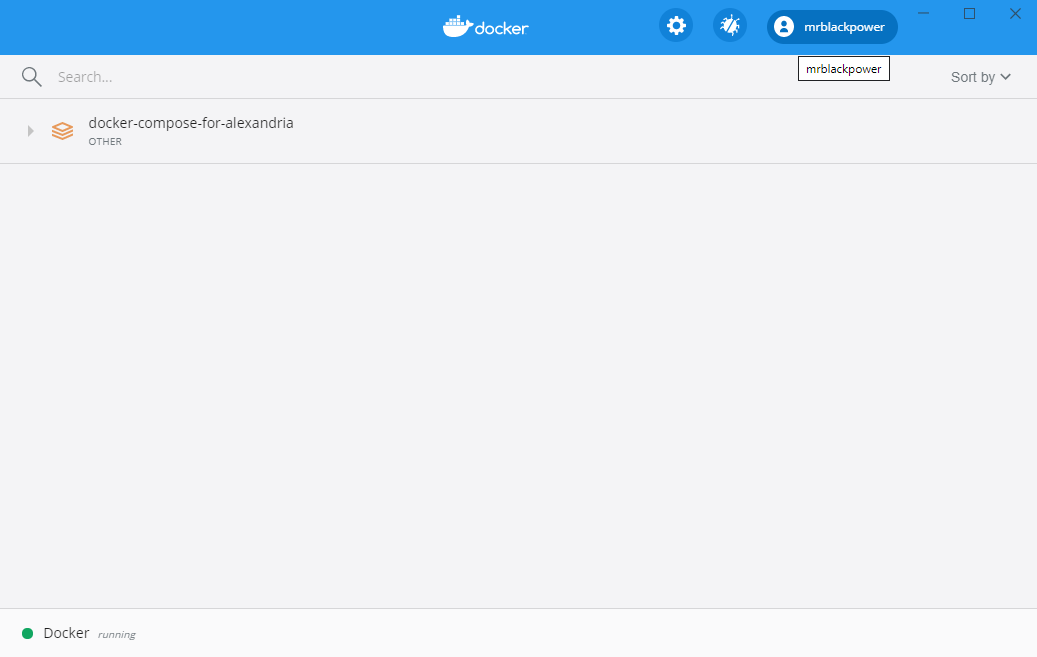
\includegraphics[width=1\textwidth]{images/16.png}
	\end{center}
	
	\framebreak
	
	\begin{itemize}
		\item Com isto é possível enviar a imagem guardada no cache do Docker para o repositório, desta forma a imagem pode ser utilizada em qualquer Docker remoto \textit{(caso seja um repositório público)}.
		
		\item \code{docker push <image:tag>}
		
	\end{itemize}
	
	\framebreak
	
	\begin{center}
		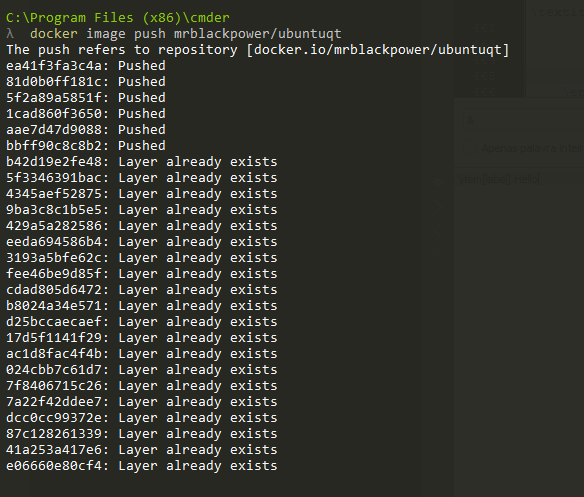
\includegraphics[width=0.7\textwidth]{images/18.png}
	\end{center}
	
	\framebreak
	
	\begin{center}
		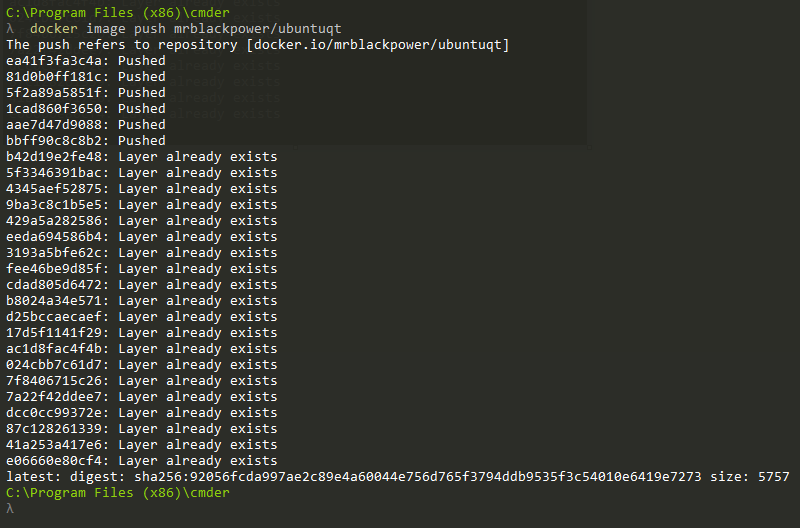
\includegraphics[width=0.7\textwidth]{images/19.png}
	\end{center}

\end{frame}

\section{Docker - Compose \& Builder}
\begin{frame}[allowframebreaks]
\frametitle{Docker - Compose \& Builder}

	\begin{itemize}
		\item O docker builder é responsável por construir contêineres através de instruções básicas.
		
		\item O comando \code{docker builder build} procura no diretório atual um arquivo \code{Dockerfile} e tenta construir o contêiner.
		
		\item O comando \code{docker builder prune} remova as camadas "sobrando".
	\end{itemize}
	
	\framebreak
	
	\begin{center}
		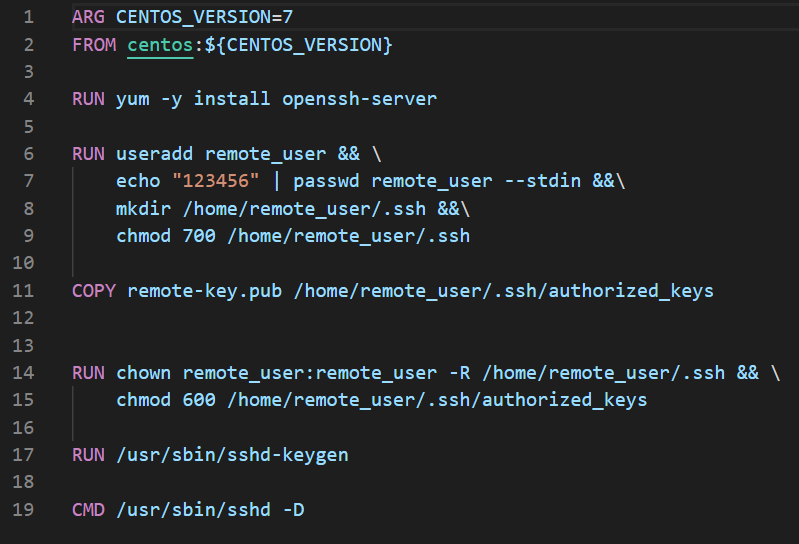
\includegraphics[width=0.7\textwidth]{images/21.png}
	\end{center}
	
	\framebreak
	
	\begin{center}
		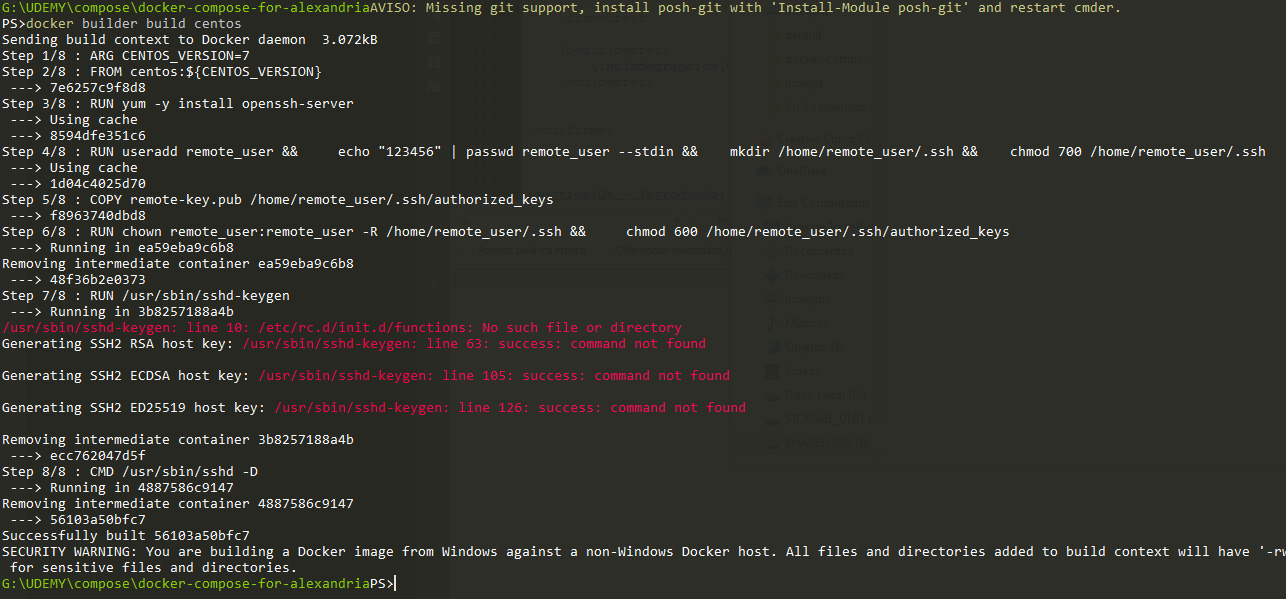
\includegraphics[width=0.7\textwidth]{images/22.png}
	\end{center}
	
	\framebreak
	
	\begin{itemize}
		\item Já o docker-compose é responsável por criar múltiplos contêineres, podendo contruí-los também no processo. É uma forma de arquitetar diversos contêineres de forma conjunta.
		\item O interessante é o compartilhamento de volumes e contêineres parametrizadosm que permitem a rápida criação de um sistema complexo de contêineres.
	\end{itemize}
	
	\framebreak
	
	\begin{center}
		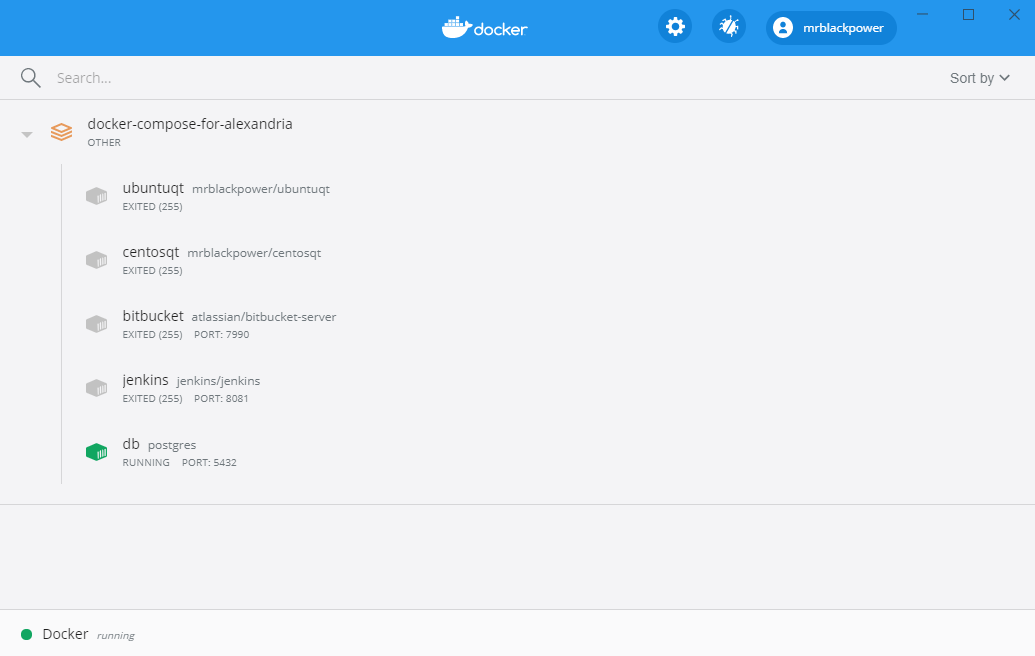
\includegraphics[width=0.7\textwidth]{images/23.png}
	\end{center}
	
	\framebreak
	
	\begin{itemize}
		\item Para utilizar o visualizar a ajuda do compose usa-se:
		
		\item \code{docker-compose --help}
		
		\item Para executar-se a construção dos contêineres é utilizado o comando abaixo somado à um arquivo YAML no mesmo diretório, usualmente \code{docker-compose.yml}.
		
		\item \code{docker-compose up -d --build}
	\end{itemize}
	
	\framebreak
	
	\begin{center}
		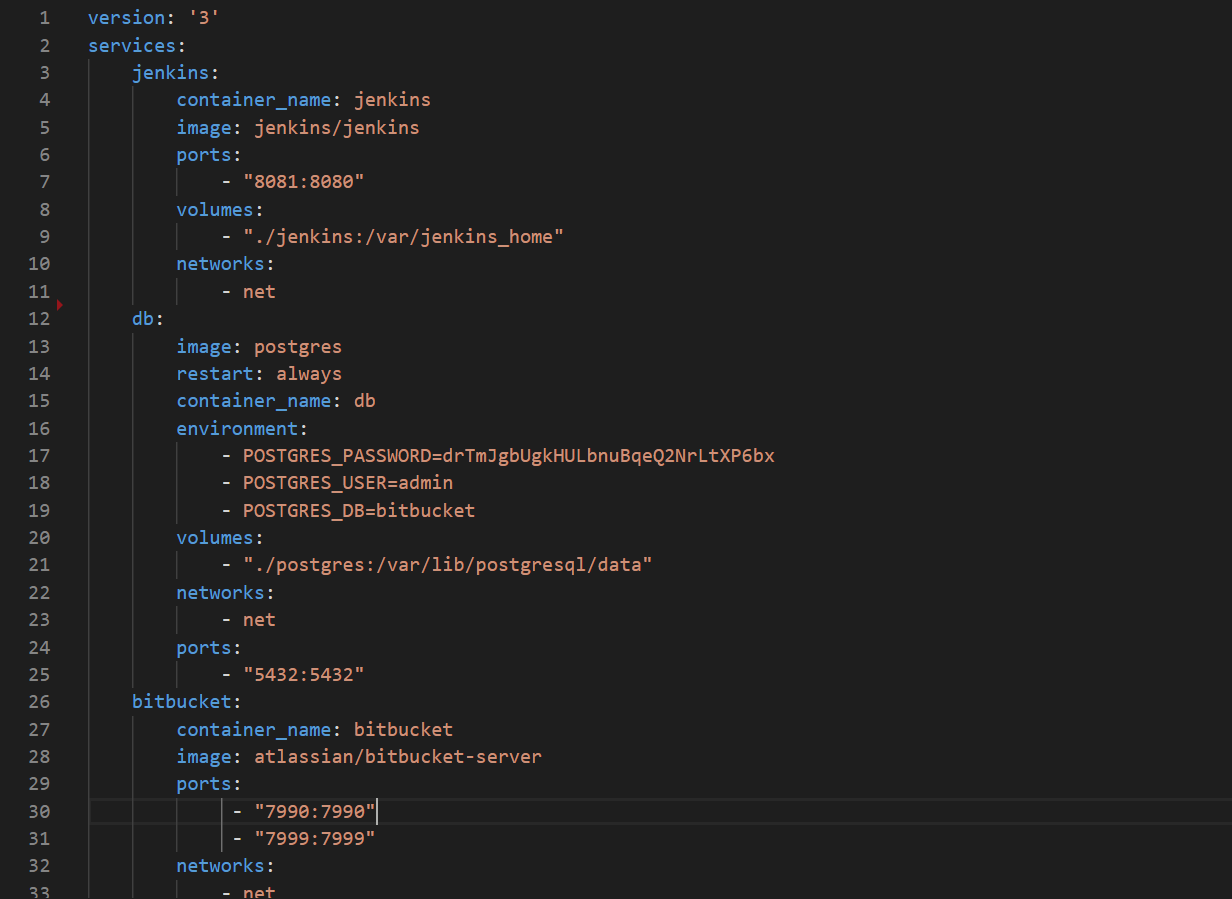
\includegraphics[width=0.7\textwidth]{images/24.png}
	\end{center}
	
	\framebreak
	
	\begin{center}
		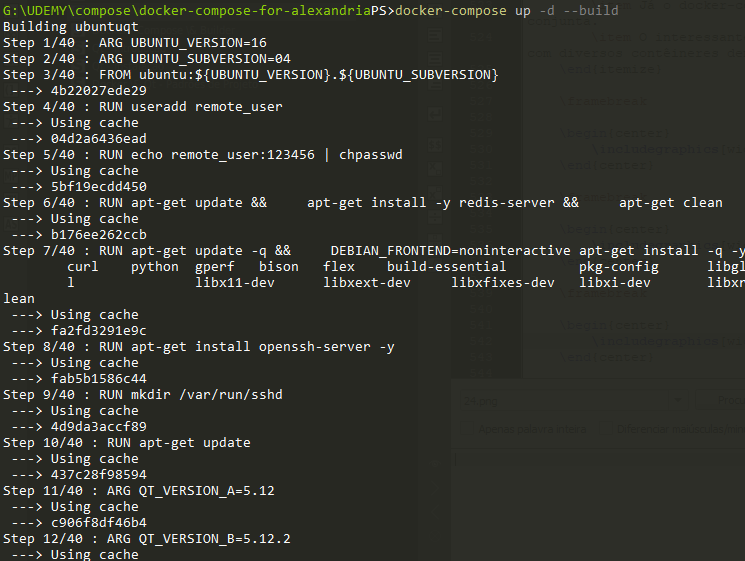
\includegraphics[width=0.7\textwidth]{images/26.png}
	\end{center}
	
	\framebreak
	
	\begin{center}
		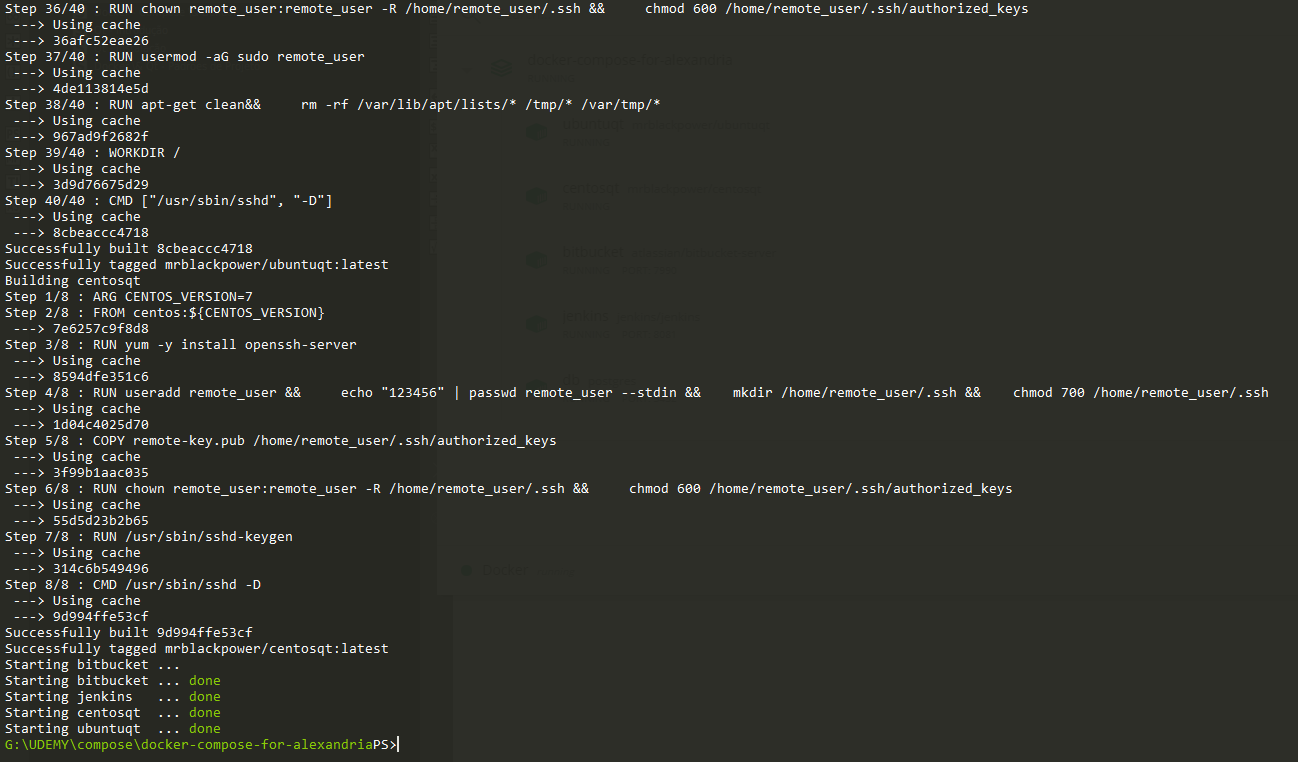
\includegraphics[width=0.7\textwidth]{images/25.png}
	\end{center}

\end{frame}



\section{Qt - Introdução}
\begin{frame}[allowframebreaks]
\frametitle{Qt - Introdução}
		
	\begin{center}
		
\includegraphics[width=0.7\textwidth]{images/12.png}
	\end{center}
	
	\framebreak

	\begin{itemize}
		\item O Qt é uma IDE (Integrated Development Environment) que possibilita a execução de programas C++ em diversos sistemas, inclusive em sistemas embarcados. O Qt era de propriedade da Nokia mas foi vendido para outra empresa (Digia) que transformou o Qt no que ele é hoje.
		
		\item Através do Qt é possível criar aplicações gráficas para diversos sistemas operacionais e diferentes sistemas embarcados. Sendo extremamente para únificação do código de projetos que utilizam de tais ambiente em um único contexto.
		

	\end{itemize}		
	
	\framebreak
		
	\begin{itemize}
		\item Dentre os programas modernos que utilizam o Qt, estão:
		
		\item Age of Wonders III (Jogo)
		
		\item Battle.net
		
		\item GNU Octave
		
		\item GMount \& Blade: Warband (Jogo)
		
		\item Spotify
		
		\item Oracle Virtualbox
		
		\item Wolfram Mathematica
	\end{itemize}

\end{frame}

\section{Qt - Instalação}
\begin{frame}[allowframebreaks]
\frametitle{Qt - Instalação}

	\begin{itemize}
		\item 	É possível se instalar as bibliotecas do Qt compilando-as, entretanto seria necessário linkar o resultado compilado manualmente ao compilador, o que é no mínimo trabalhoso.
		\item É recomendado que se instale o Qt utilizando o instalador do Qt (em qualquer SO). Um fato interessante é que o próprio instalador do Qt é desenvolvido em cima das bibliotecas do Qt.
		\item O instalador ainda pode ser utilizado sem a interface gráfica, o que facilita sua utilização dentro de contêineres do Docker.
	\end{itemize}
	
	
	\framebreak
	
	\begin{center}
		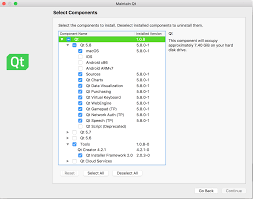
\includegraphics[width=0.7\textwidth]{images/20.png}
	\end{center}
	
	\framebreak
	
	\begin{itemize}
		\item Uma vez instaladas corretamente, as bibliotecas serão acessíveis e o software de programação QtCreator é instalado juntamente.
		
		\item O QtCreator é atualmente uma das grandes ferramentas utilizadas no desenvolvimento de aplicações em C++ e funciona também para projetos que não incluem as bibliotecas do Qt.
		
		\item Outro comando instalado juntamente é o \code{qmake}, este comando funciona de modo similar ao \code{cmake}, configurando os arquivos para serem compilados e linka a interface gráfica.
		
		\item A grande vantagem destas bibliotecas está no fato de que podem ser instaladas em quase qualquer ambiente computacional e funciona utilizando os mesmos passos. Uma vez executado o \code{qmake} é possível compilar todo o projeto com qualquer compilador C++. Para projetos com interface gráfica isto é uma grande vantagem pois cada SO lida com protocolos diferentes para exibição de imagens ou mesmo os componentes da interface gráfica e o Qt unifica todos estes comandos.
	\end{itemize}
	
	\framebreak
	
	\begin{center}
		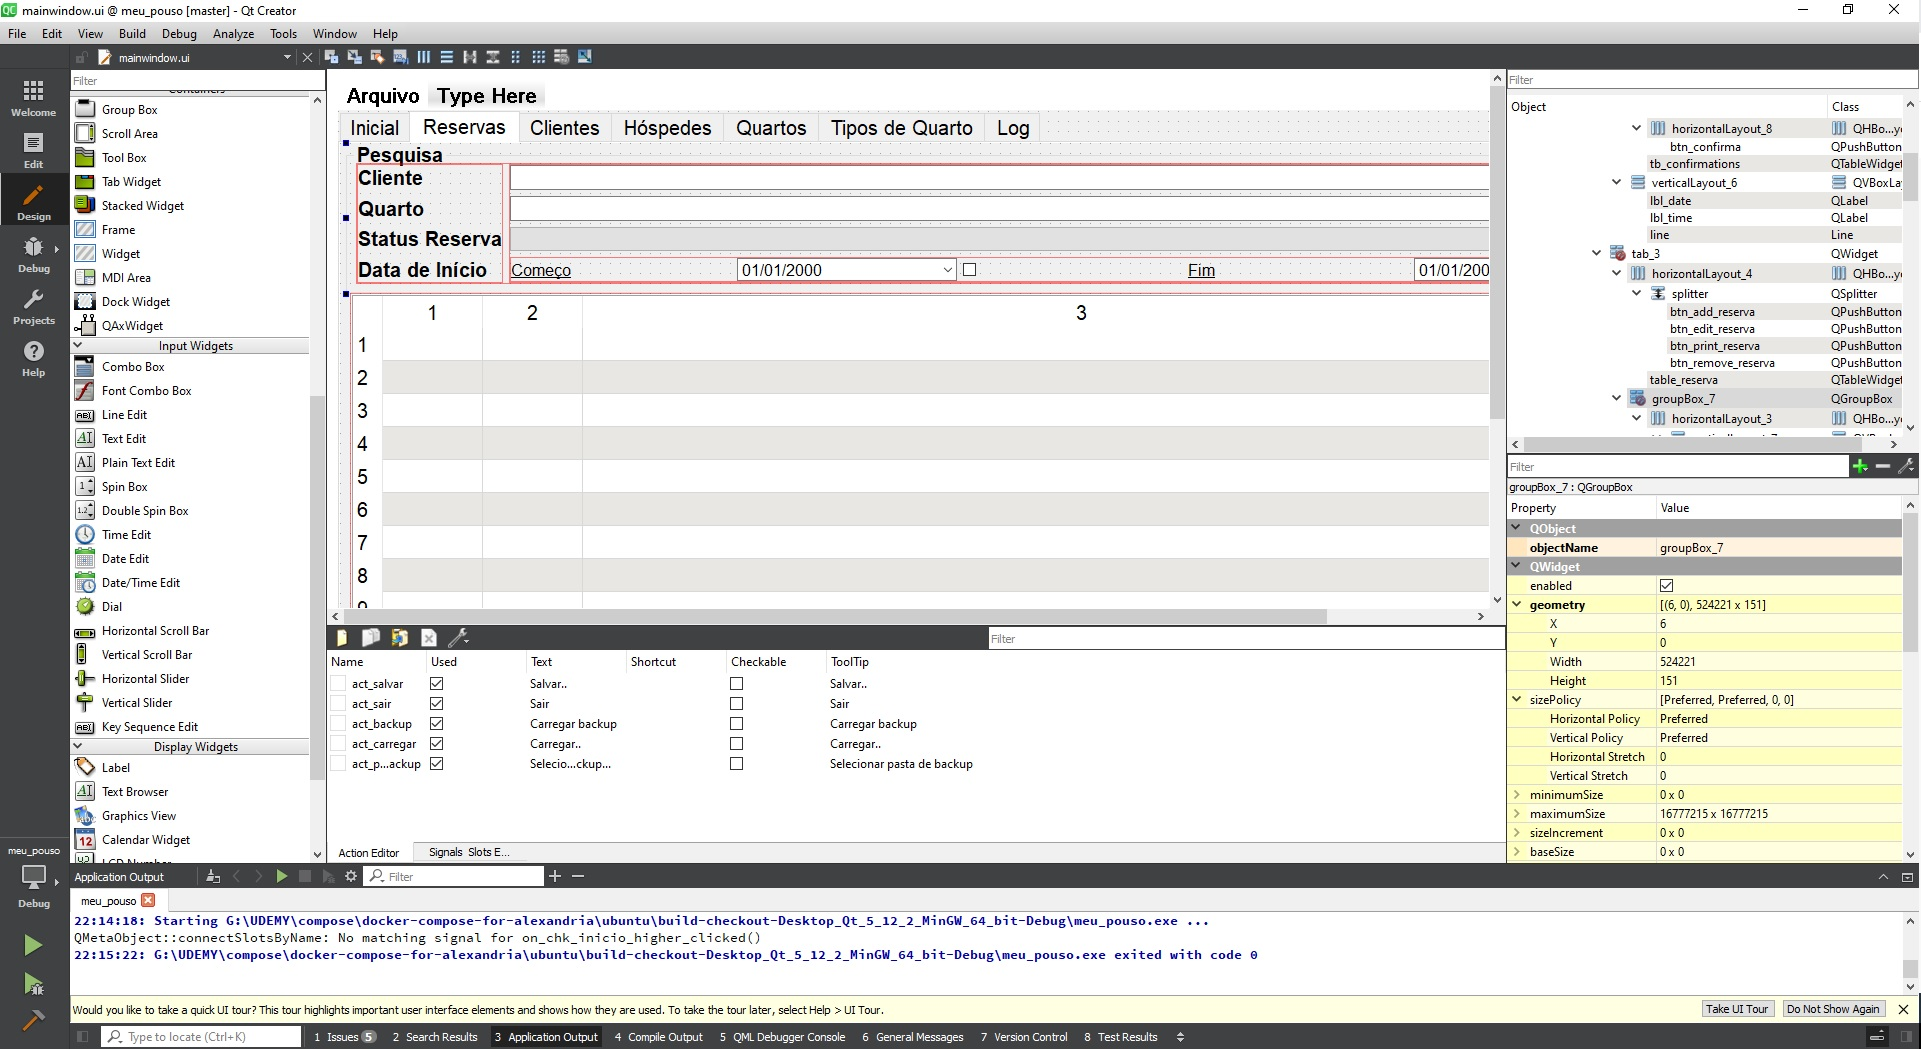
\includegraphics[width=0.7\textwidth]{images/04.jpg}
	\end{center}

\end{frame}

\section{Qt - Interface Gráfica}
\begin{frame}[allowframebreaks]
\frametitle{Qt - Interface Gráfica}

	\begin{itemize}
		\item Através do próprio QtCreator é possível se criar projetos com interface de usuário gráficas utilizando os chamados QtWidgets.
	\end{itemize}
	
	\begin{center}
		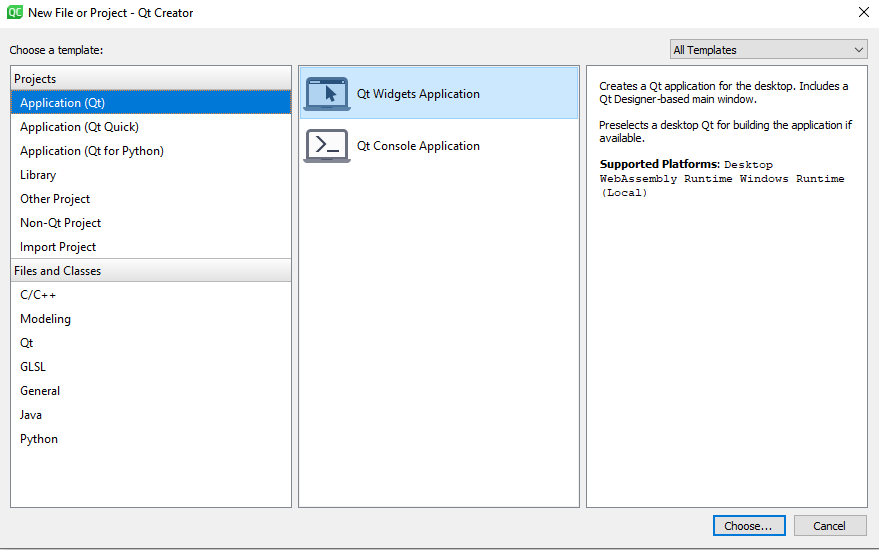
\includegraphics[width=0.7\textwidth]{images/27.png}
	\end{center}
	
	\framebreak
	
	\begin{itemize}
		\item É possível ainda selecionar a "máquina" construtora (qmake ou cmake).
	\end{itemize}
	
	\begin{center}
		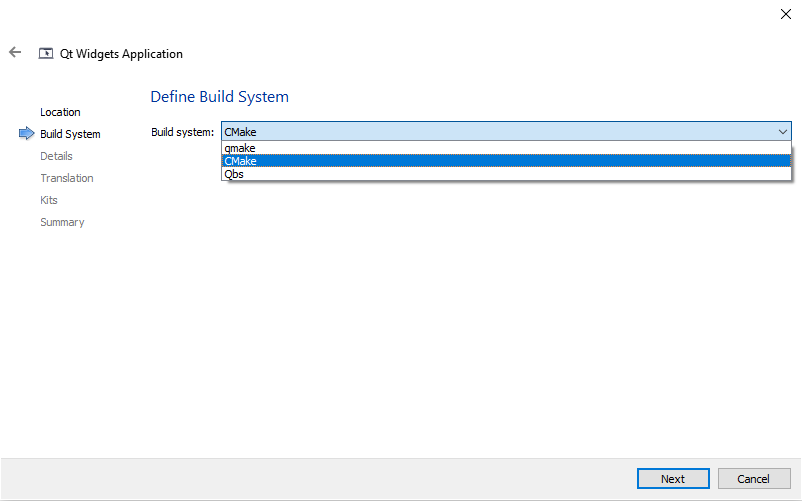
\includegraphics[width=0.7\textwidth]{images/28.png}
	\end{center}
	
	\framebreak
	
	\begin{itemize}
		\item É necessário inserir o nome da janela principal e o seu tipo. O tipo QMainWindow representa uma janela principal, passível de ser utilizada na maioria das aplicações. Sendo composta por três arquivos \code{.h .cpp .ui}, sendo o último responsável por conter os elementos da interface gráfica.
	\end{itemize}
	
	\begin{center}
		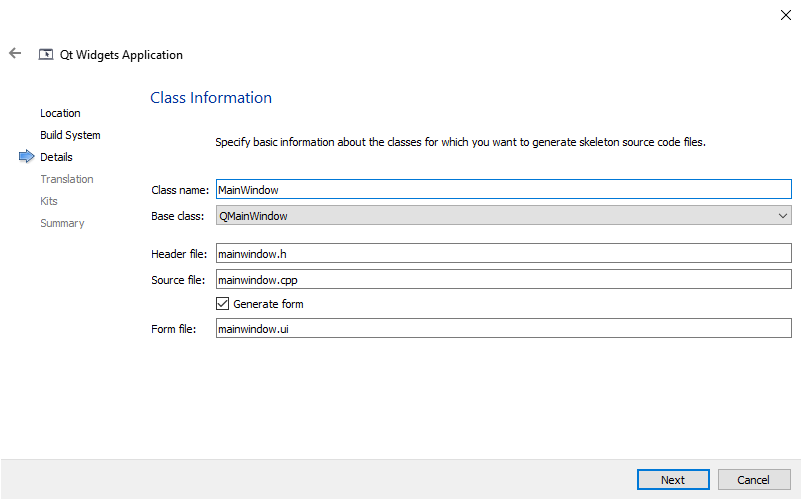
\includegraphics[width=0.7\textwidth]{images/29.png}
	\end{center}
	
	\framebreak
	
	\begin{center}
		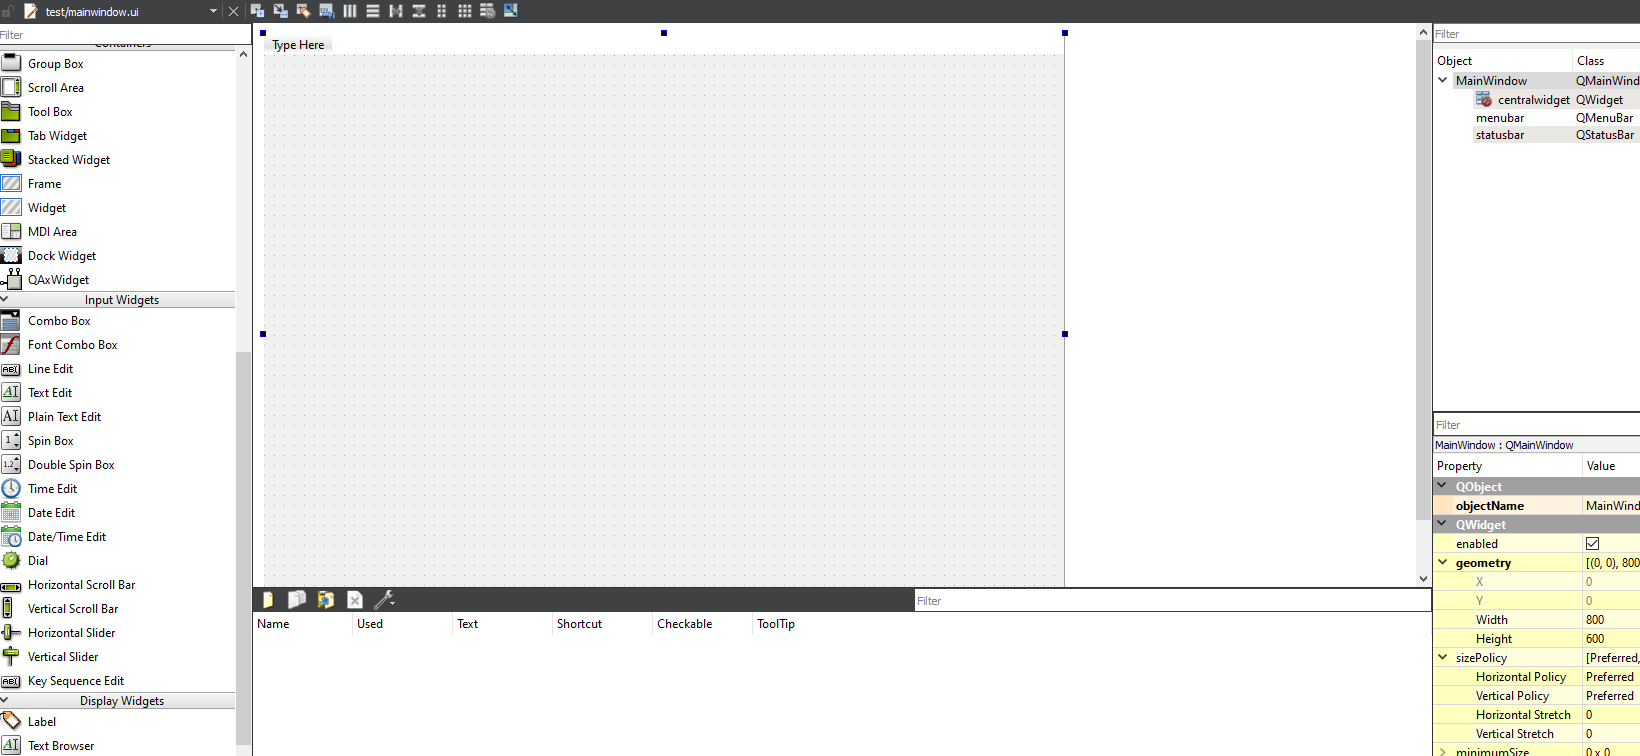
\includegraphics[width=0.7\textwidth]{images/31.png}
	\end{center}
		
	\framebreak

	\begin{itemize}
		\item É possível ver a estrutura principal do programa acessando o arquivo main.cpp que continua sendo o arquivo principal do projeto. Aqui vemos Um objeto que representa a janela principal sendo criado e exibido, enquanto uma aplicação recebe os agumentos de entrada e é enviado no retorno.
		
		\item Na realidade esta aplicação representa o loop do programa, que eventualmente passa pela janela por ser um loop especial, mas não fica travado nele.
	\end{itemize}
	
	\begin{center}
		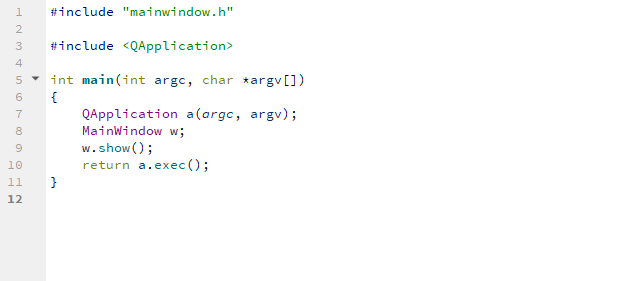
\includegraphics[width=0.7\textwidth]{images/30.png}
	\end{center}
		
	\framebreak
	
	\begin{itemize}
		\item Ao executar a ferramenta de configuração (cmake ou qmake) as bibliotecas do Qt são acionadas e os três arquivos (.cpp .h e .ui) são linkados
		
		\item Na realidade, por debaixo dos panos o Qt cria outras classes de interface baseadas no arquivo .ui e as compila. O Qt é responsável por essa tradução e por este motivo que ao modificar a interface é possível que erros C++ apareçam na compilação.
	\end{itemize}
\end{frame}


\section{Docker \& Qt - Padrões de Projeto}
\begin{frame}[allowframebreaks]
\frametitle{Docker \& Qt - Padrões de Projeto}

	\begin{itemize}
		\item O Qt pode ser compilado para diferentes plataformas e possui diferentes versões com diferentes funcionalidades.
		
		\item Portanto, o Docker fornece um ambiente estável para que o programa seja compilado e lançado(deployed).
		
		\item Ainda dentro do Docker é possível manter um repositório local e um automatizador.
		
		\item Para estas funções foram escolhidos, respectivamente o Bitbucket Server e o Jenkins.
	\end{itemize}
	
	\framebreak
	
	\begin{center}
		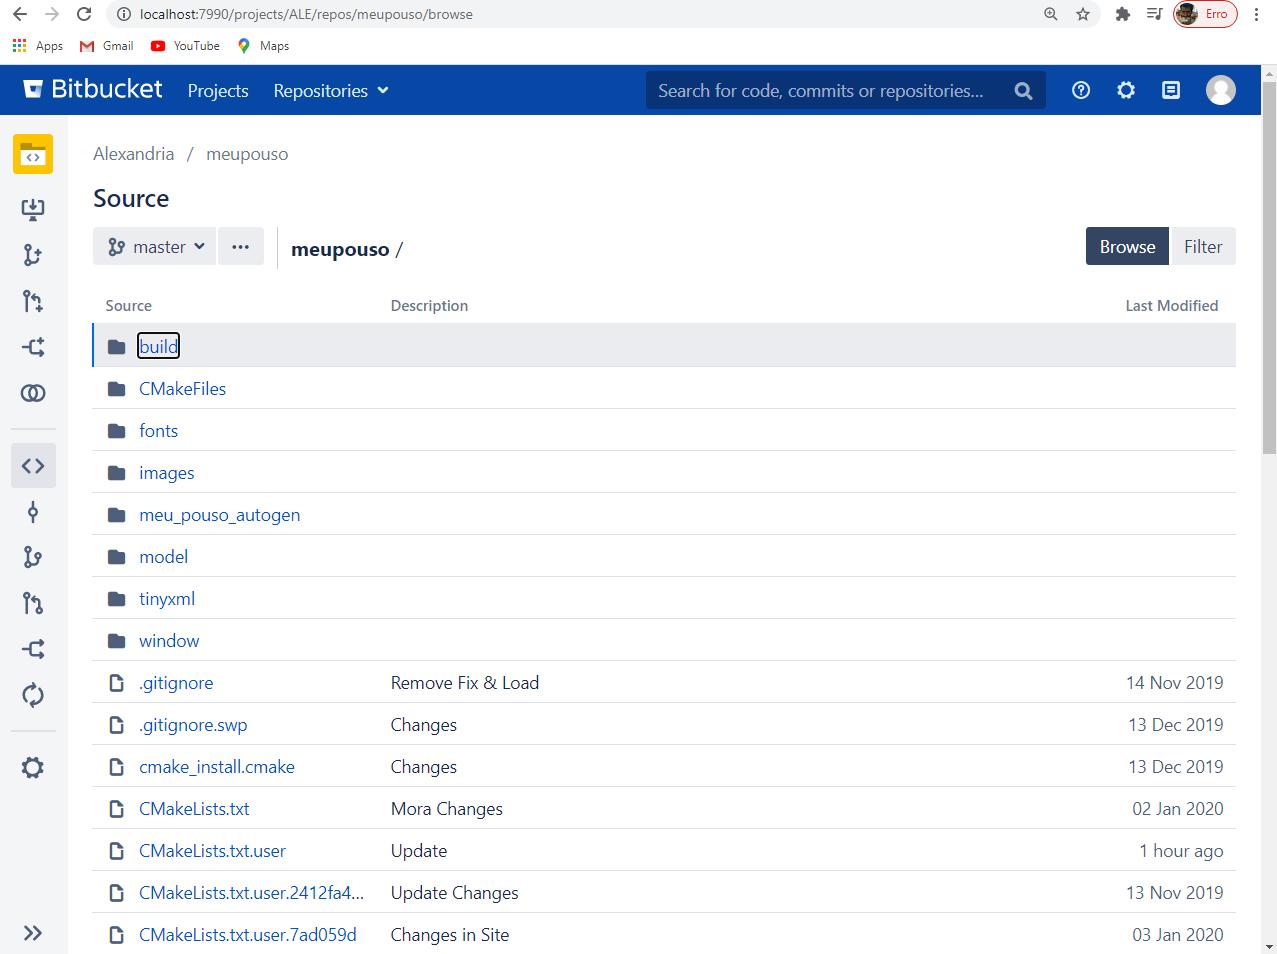
\includegraphics[width=0.7\textwidth]{images/32.png}
	\end{center}
	
	\framebreak
	
	\begin{center}
		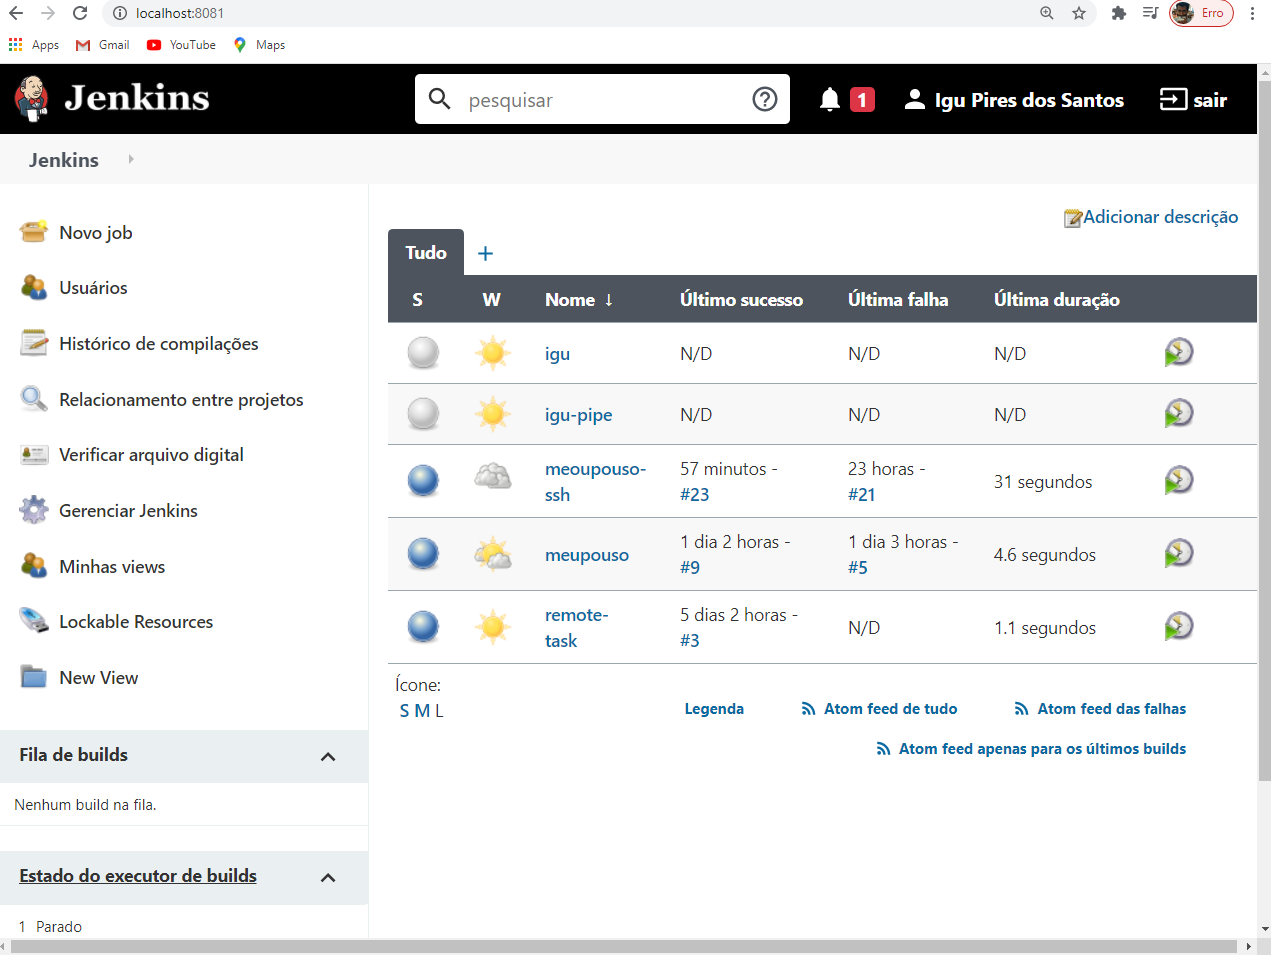
\includegraphics[width=0.7\textwidth]{images/37.png}
	\end{center}
	
	\framebreak
	
	\begin{center}
		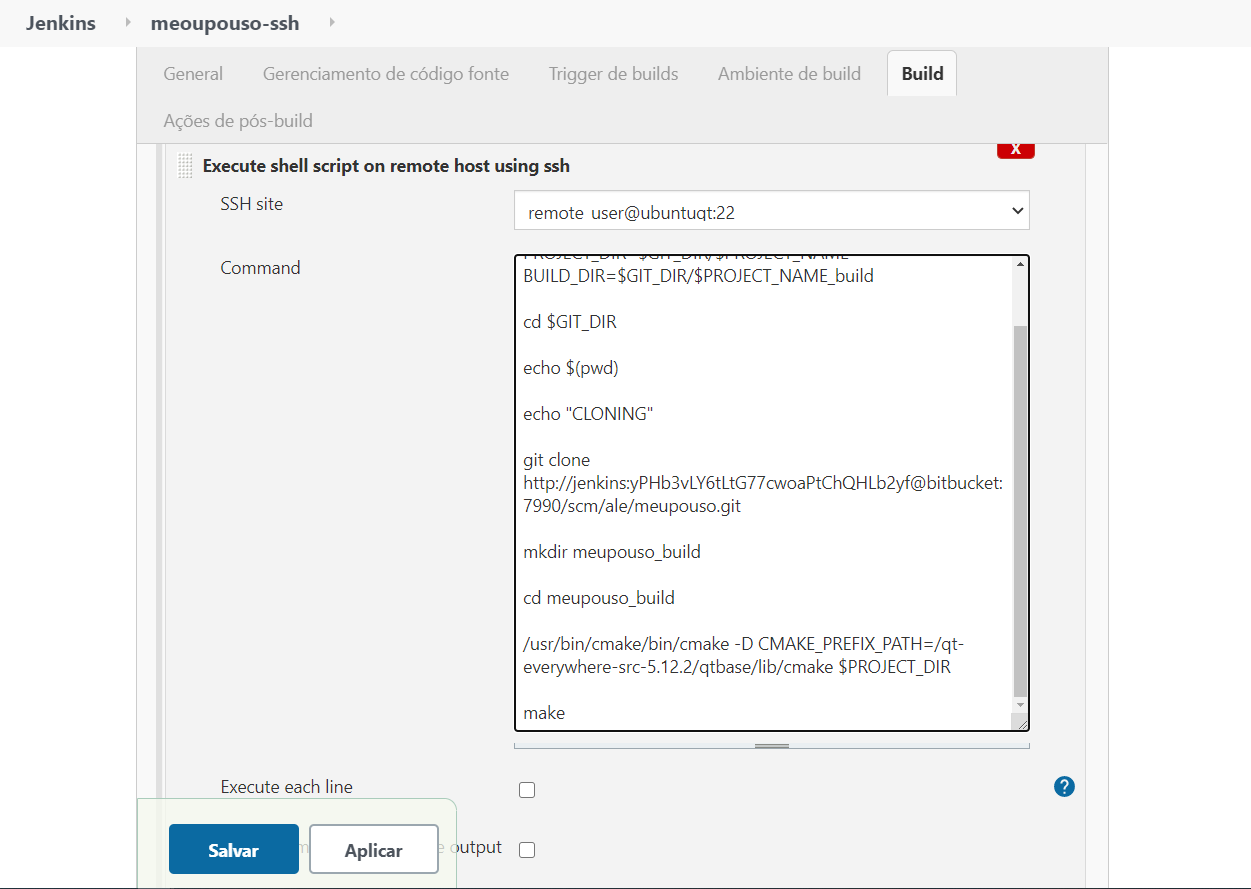
\includegraphics[width=0.7\textwidth]{images/33.png}
	\end{center}
	
	\framebreak
	
	\begin{center}
		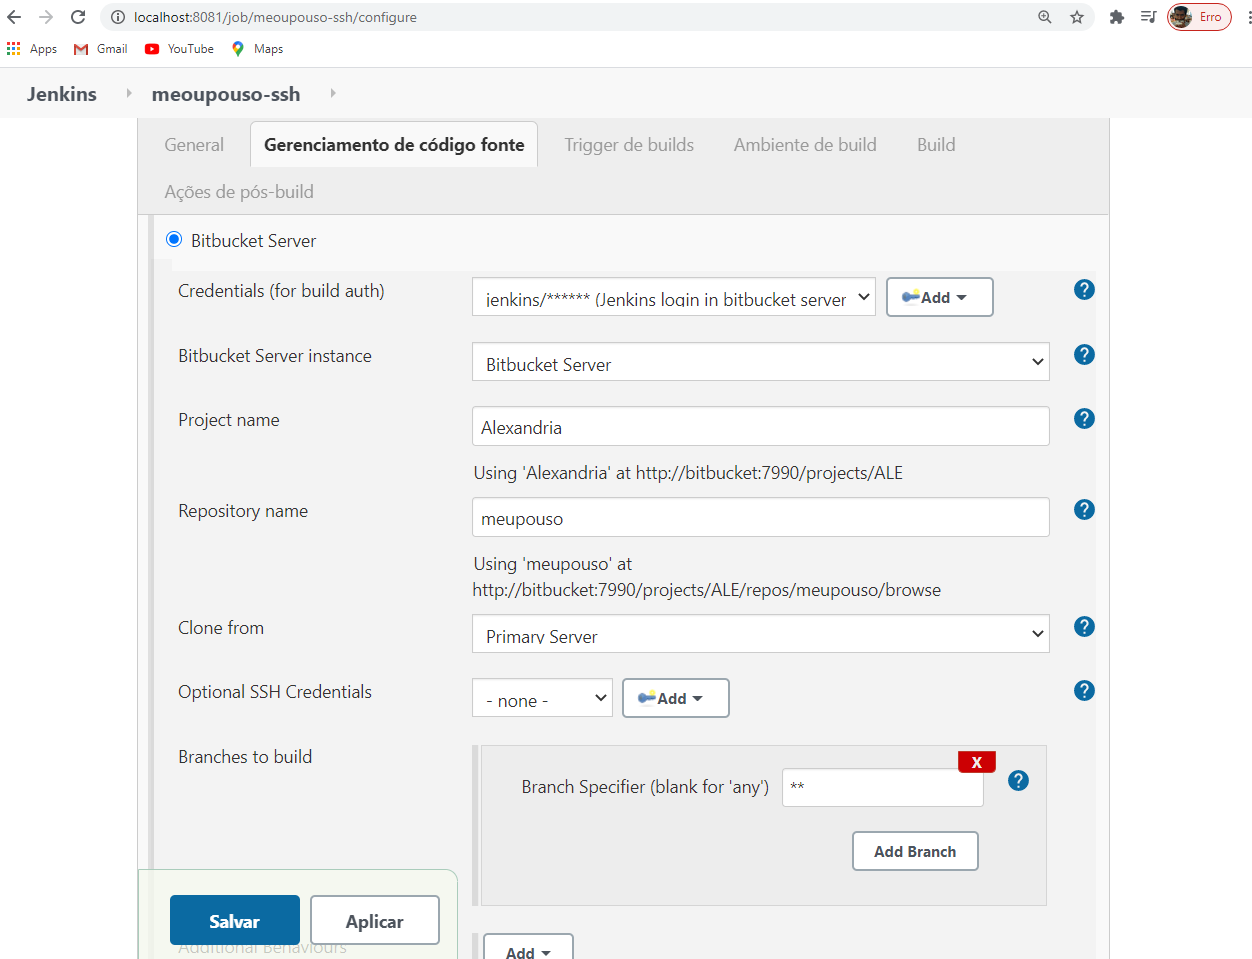
\includegraphics[width=0.7\textwidth]{images/34.png}
	\end{center}
	
	\framebreak
	
	\begin{center}
		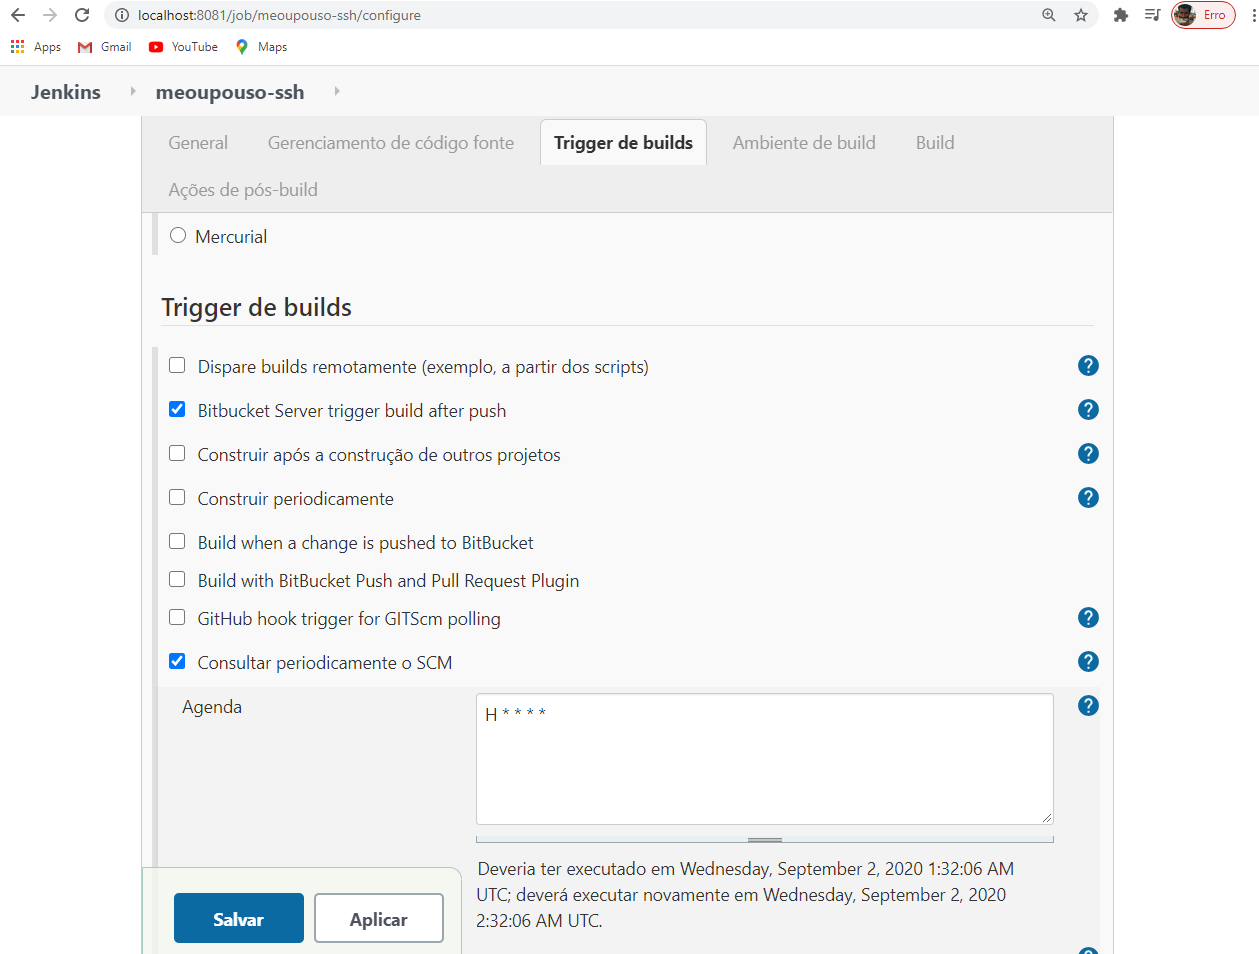
\includegraphics[width=0.7\textwidth]{images/35.png}
	\end{center}
	
	\framebreak
	
	\begin{center}
		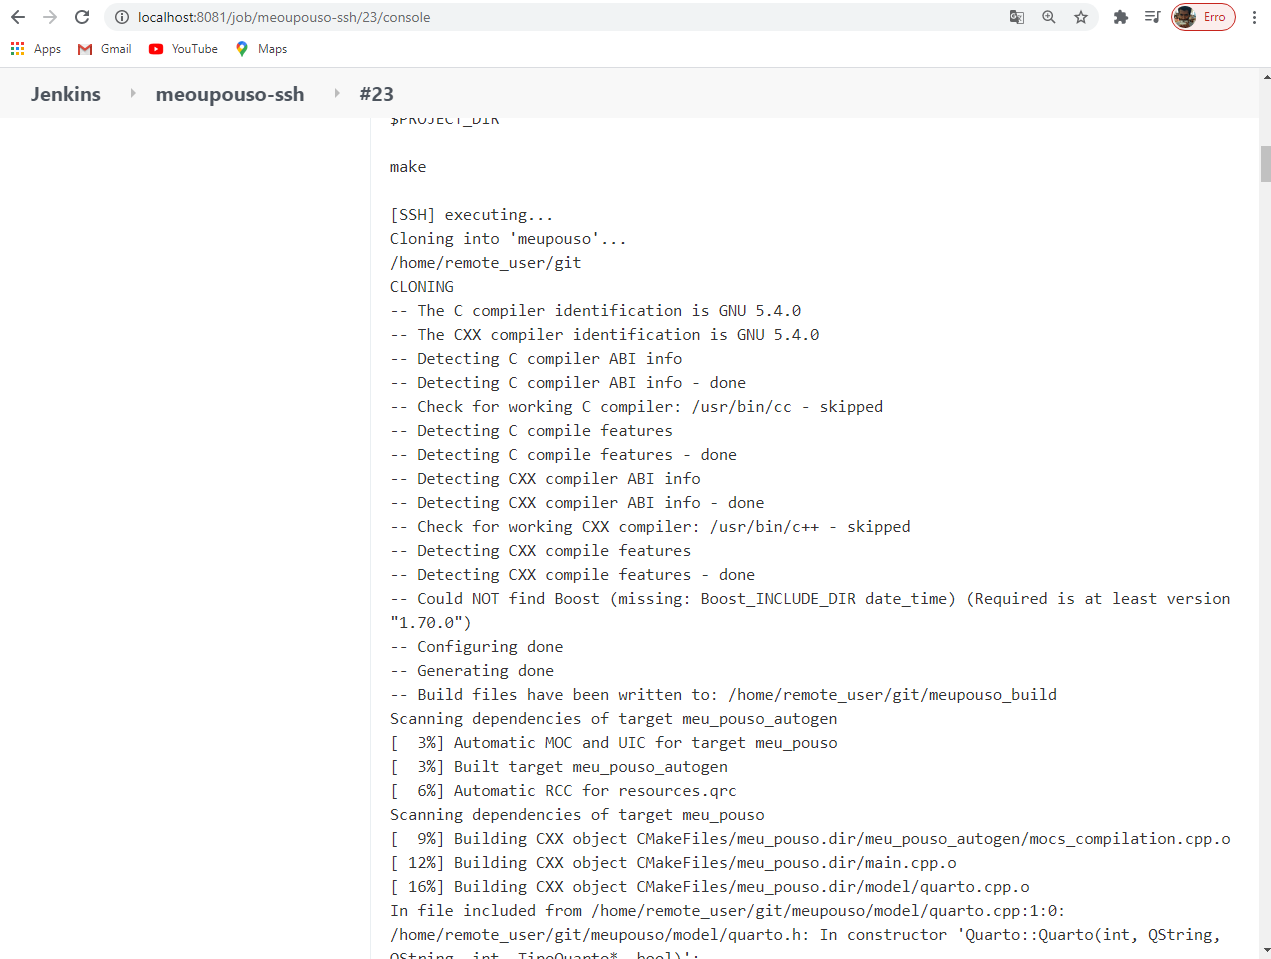
\includegraphics[width=0.7\textwidth]{images/36.png}
	\end{center}
	
	\framebreak
	
	\begin{itemize}
		\item Sumarizando, são 3 contêineres principais, um com o SO de lançamento (deploy), um com o repositório (Bitbucket) e um com o automatizador (Jenkins)
		
		\item (Demonstrar no ambiente)
	\end{itemize}
	
	\framebreak
	
	\begin{center}
		\textbf{Obrigado!}
	\end{center}

\end{frame}
\end{document}
